\fakesection{Unsupervised Learning and Large Scale Problems}{\hfill\small\texttt{/src/session\_3.m}, \texttt{/src/homework\_3.m}}

\fakesubsection{Kernel principal component analysis}{}

The point of \textit{linear principal component analysis (PCA)} is to find a linear transformation (a projection onto an orthogonal basis) such that the variance of the projected data points is maximised. It's an old method introduced by Pearson. The transformed variables are called principal components. By disregarding some of these it is possible to achieve a dimensionality reduction while still capturing most of the important information carried by the input data. This can be used for denoising purposes.

\begin{figure}[h]
\centering
%
\subfloat[De-noising with linear PCA.]{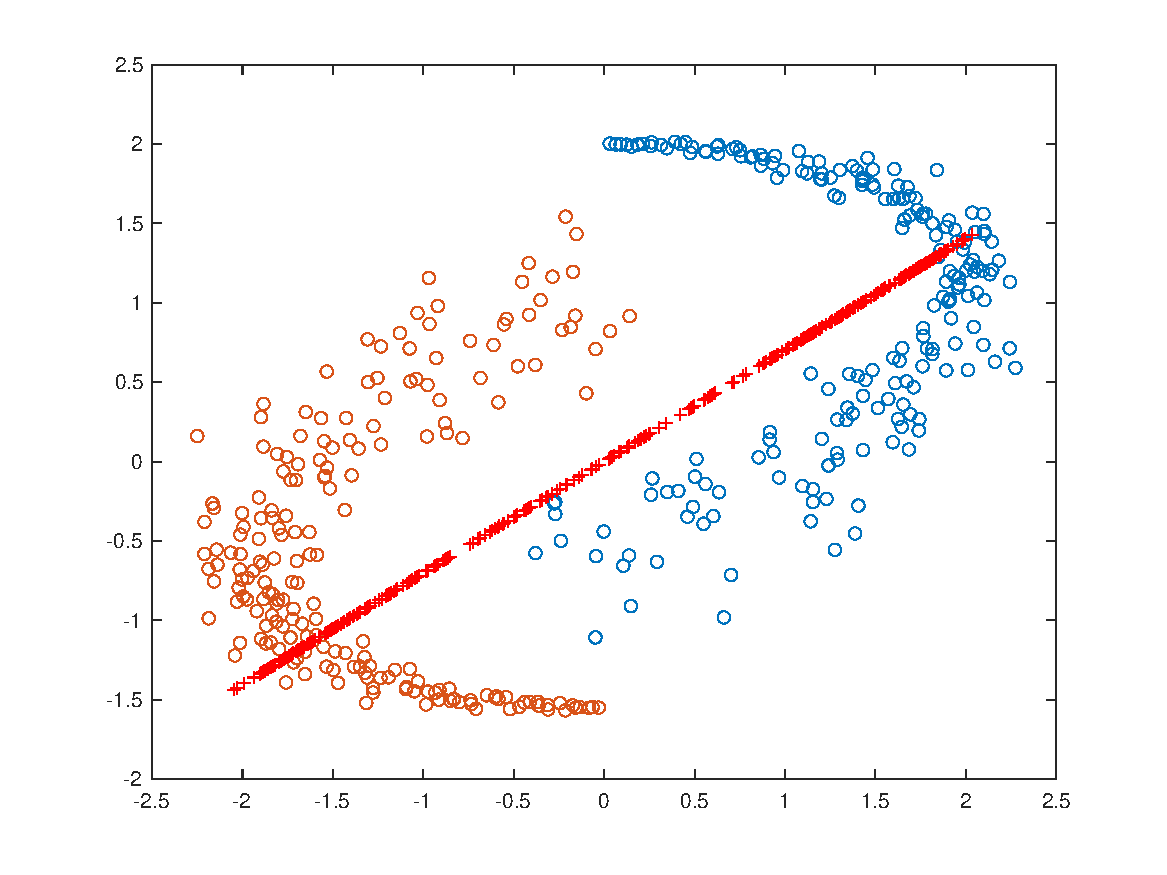
\includegraphics[width=0.35\textwidth]{../src/figures/kpca/linear}}\\
%
\subfloat[$\sigma^2=0.4,n_h=2$.]{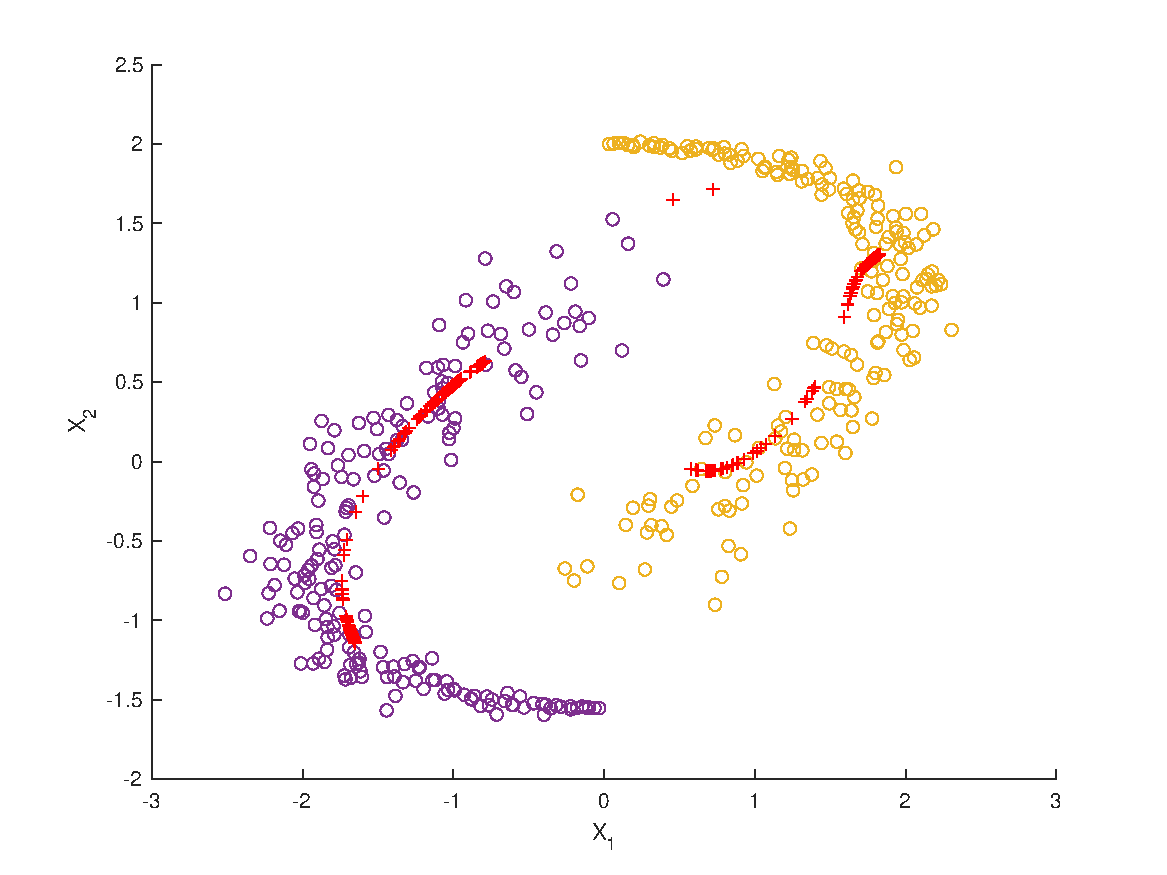
\includegraphics[width=0.25\textwidth]{../src/figures/kpca/kpca_2}}\quad
\subfloat[$\sigma^2=0.4,n_h=6$.]{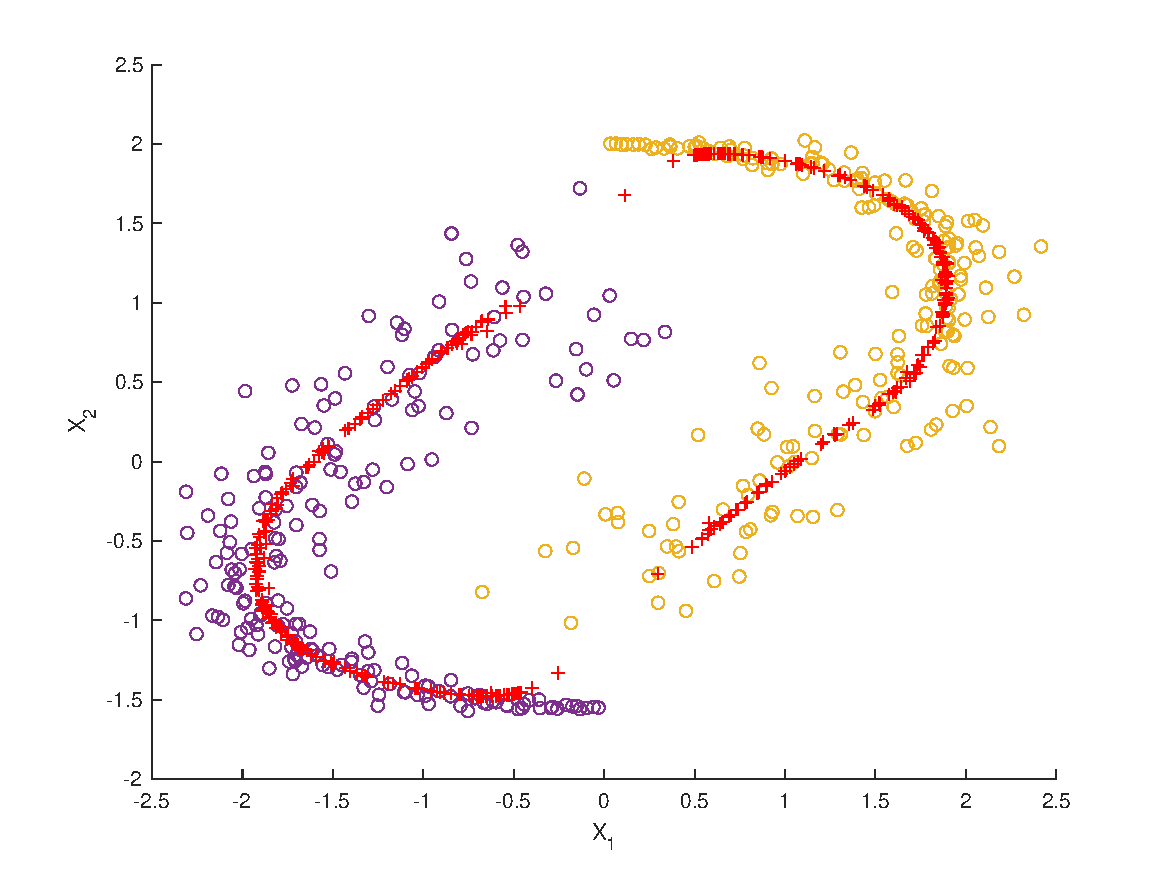
\includegraphics[width=0.25\textwidth]{../src/figures/kpca/kpca_6}}\quad
\subfloat[$\sigma^2=0.4,n_h=20$.]{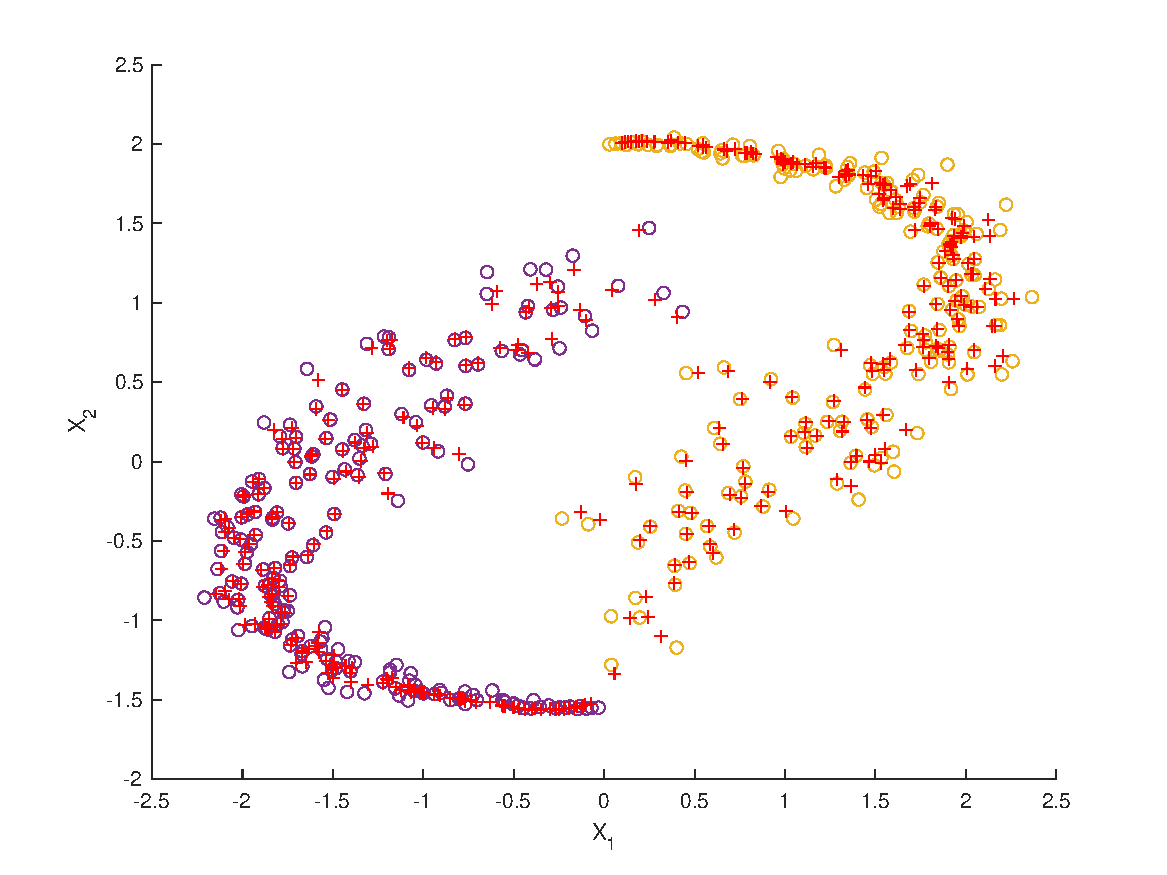
\includegraphics[width=0.25\textwidth]{../src/figures/kpca/kpca_20}}\\
%
\subfloat[$\sigma^2=1.0,n_h=2$.]{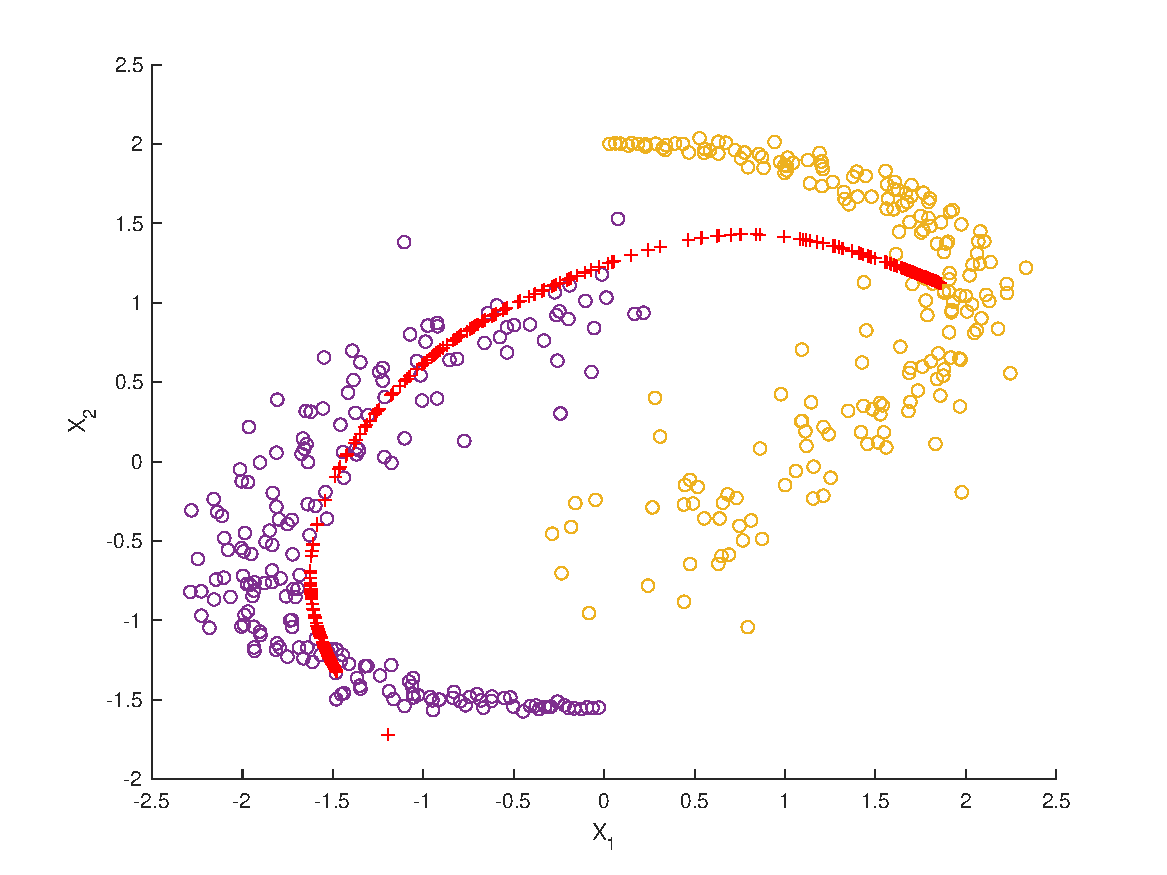
\includegraphics[width=0.25\textwidth]{../src/figures/kpca/kpca_bis_2}}\quad
\subfloat[$\sigma^2=1.0,n_h=6$.]{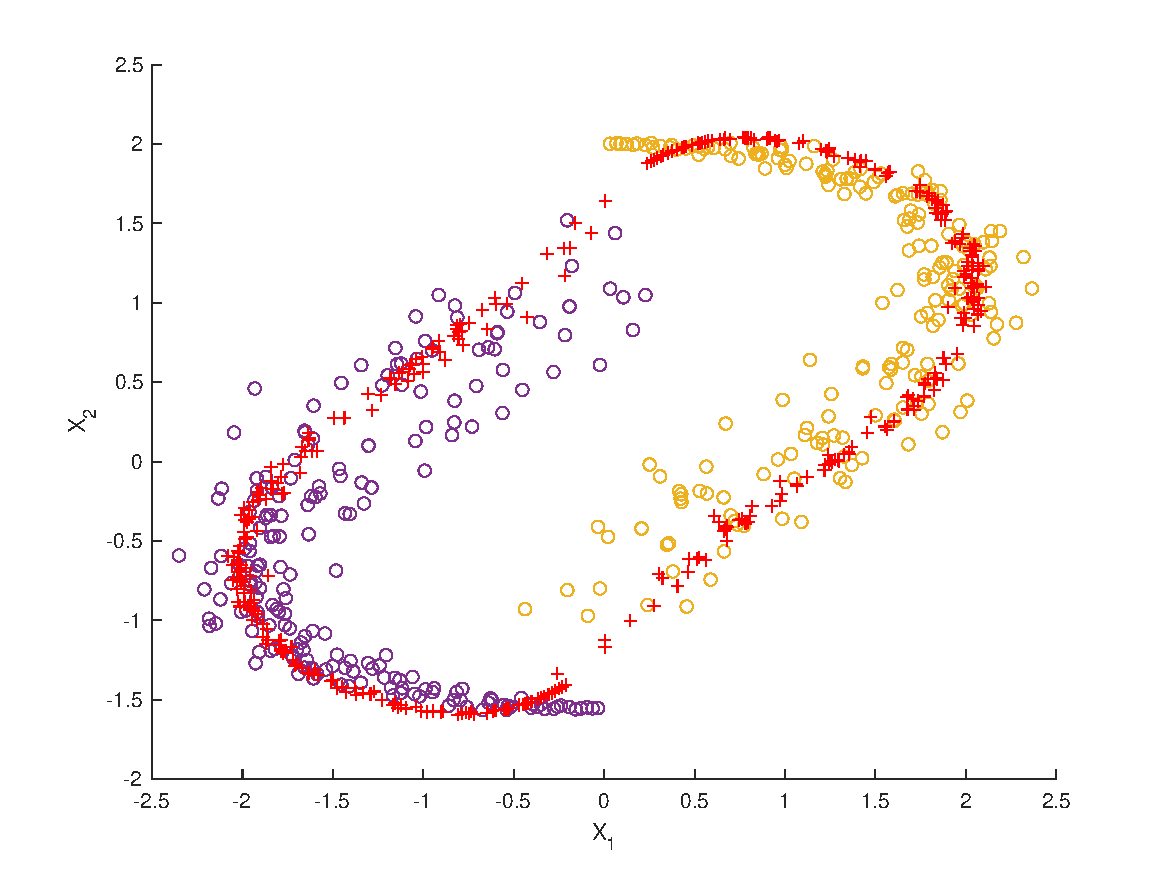
\includegraphics[width=0.25\textwidth]{../src/figures/kpca/kpca_bis_6}}\quad
\subfloat[$\sigma^2=1.0,n_h=20$.]{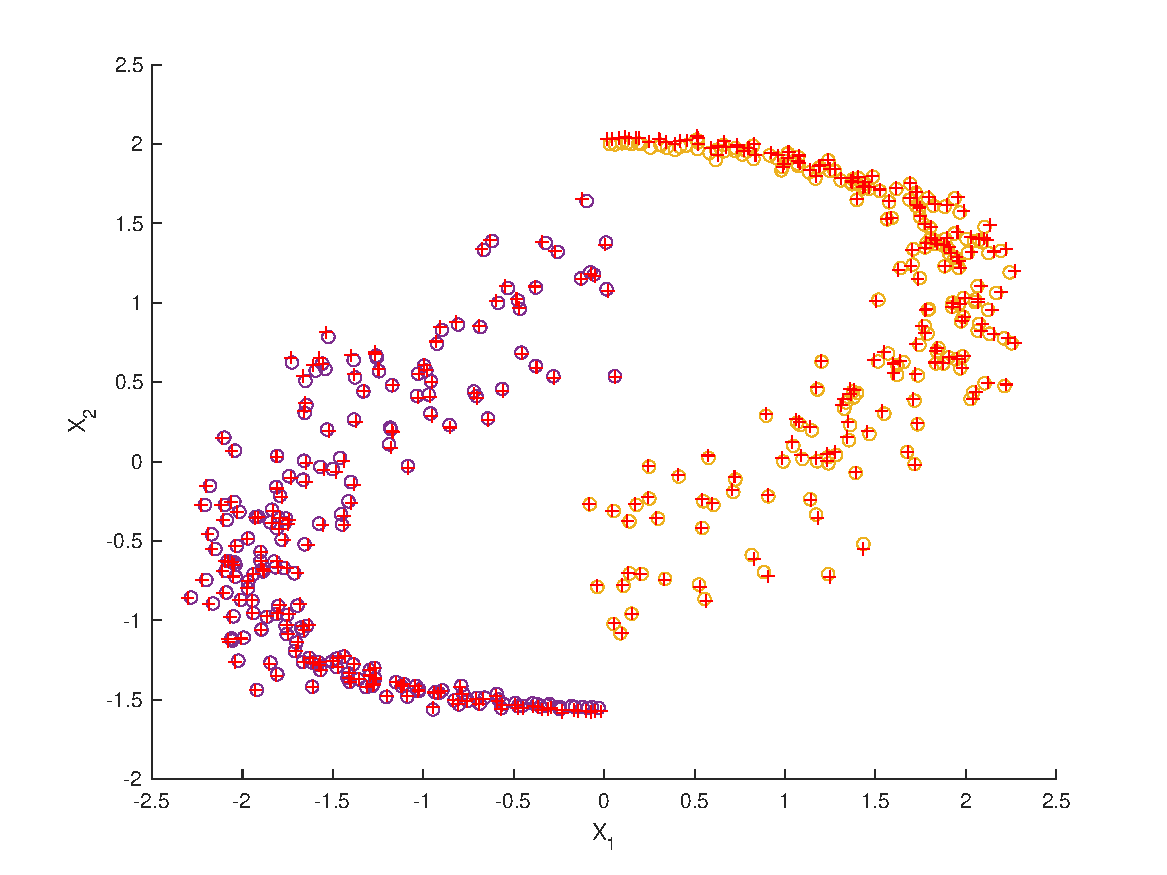
\includegraphics[width=0.25\textwidth]{../src/figures/kpca/kpca_bis_20}}\\
%
\subfloat[$\sigma^2=10.0,n_h=2$.]{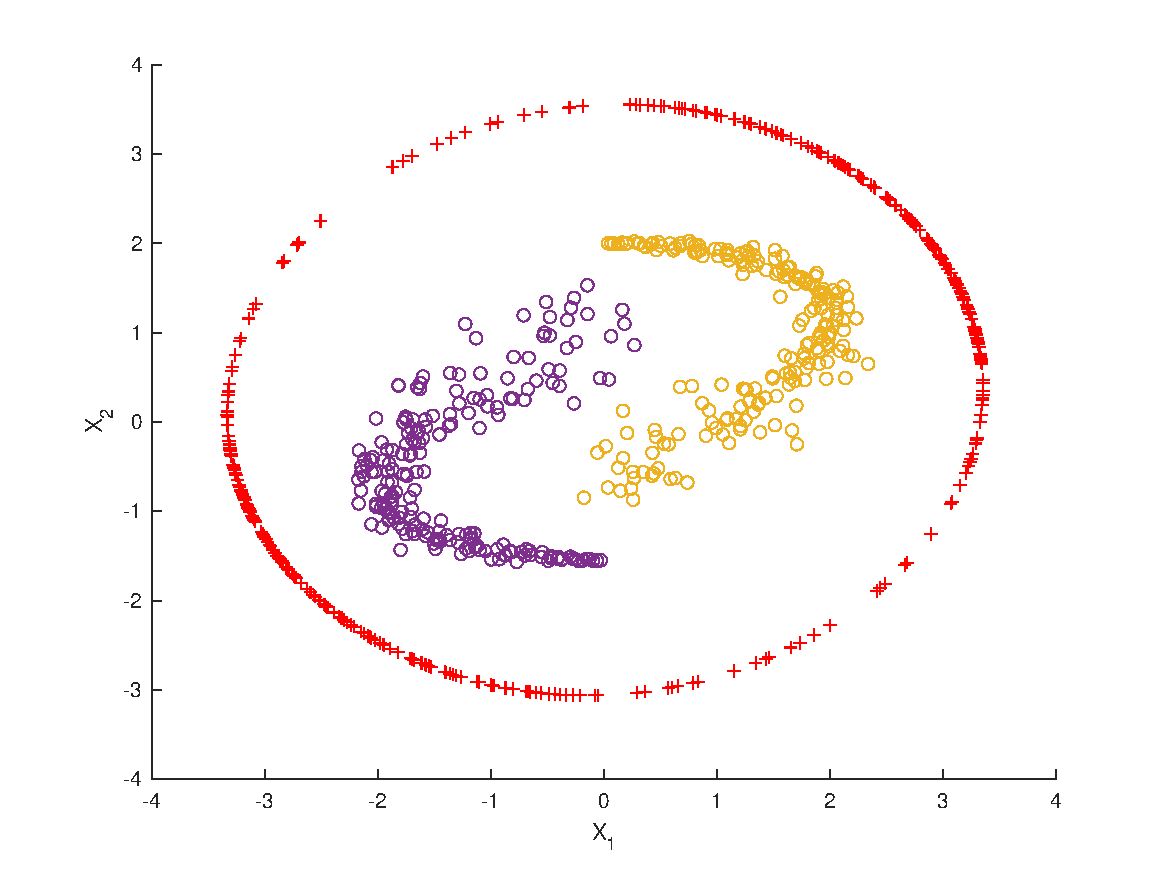
\includegraphics[width=0.25\textwidth]{../src/figures/kpca/kpca_tris_2}}\quad
\subfloat[$\sigma^2=10.0,n_h=6$.]{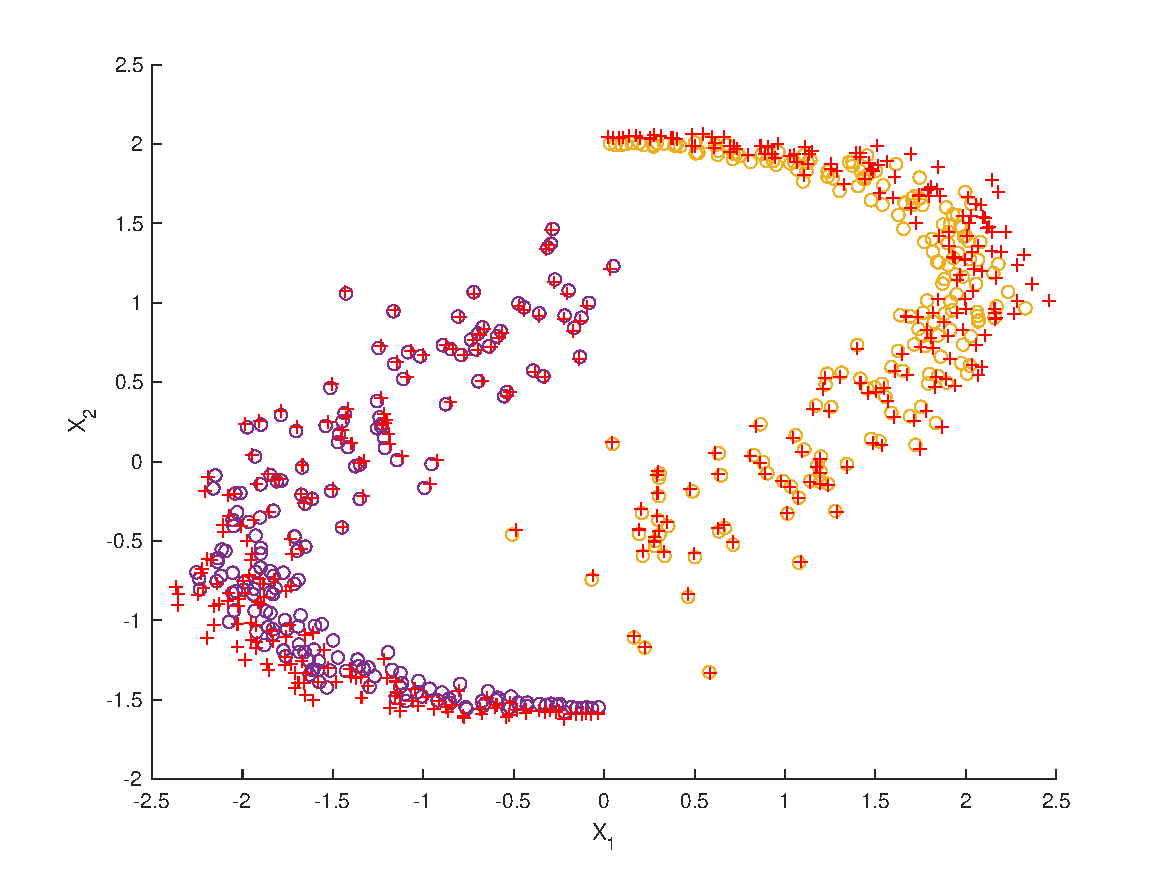
\includegraphics[width=0.25\textwidth]{../src/figures/kpca/kpca_tris_6}}\quad
\subfloat[$\sigma^2=10.0,n_h=20$.]{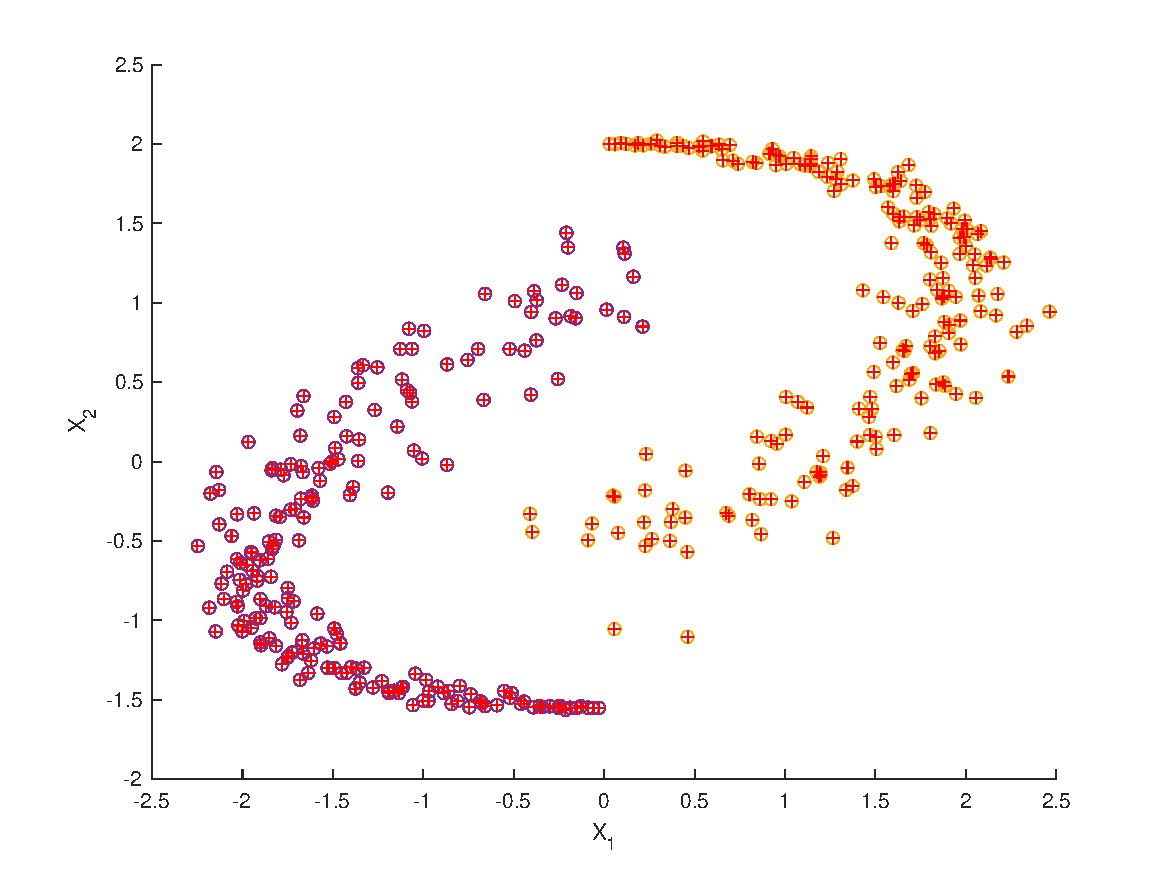
\includegraphics[width=0.25\textwidth]{../src/figures/kpca/kpca_tris_20}}\\
%
\caption{De-noising a toy dataset consisting of two spirals. The number of data points equals 400, the data point dispersion 0.3. $n_h$ is the number of components. All 9 images below the top one use an RBF kernel. De-noising is done by minimising the distance between the feature mapping of an input and its projection in the feature space onto principal axes. Retaining too few principal components leads to a poor result while retaining too many of them prevents any de-noising.}
\label{kpcatoy}
\end{figure}

\par Like Fisher discriminant analysis (FDA) it is possible to relate this to LS-SVMs and formulate it as a constraint optimisation problem :
$$\max_{w,e}\quad\mathcal{J}_P(w,e)=\gamma\frac{1}{2}\sum_{k=1}^Ne_k^2-\frac{1}{2}w^Tw\qquad\text{such that $e_k=w^T\cdot x_k\quad(k=1,\dots, N)$}$$
The errors represent the variance after projection which is to be maximised. Here too, a dual form can be introduced using Lagrange multipliers. This makes it possible to apply the kernel trick which can make for a non-linear approach (in which case PCA is applied in the feature space). Additionally an increase in the number of dimensions becomes possible when the number of training samples is larger than the number of dimensions. The bias term is responsible for centering the kernel matrix automatically rather than having to do this beforehand. This is especially interesting in the case of kernel spectral clustering (KSC) which is considered in the next paragraph and where centring is not a straightforward thing to do.

\par Because the alternative PCA formulation is model-based it becomes possible to do so-called out-of-sample extensions - the solution is not limited to the input data. It also becomes possible to tune models and find the right parameters that fit the data. However, because of the unsupervised nature of PCA this is not trivial. If the resulting model is meant to be used as a sort of preprocessing step e.g. for use in classification or in the context of a reconstruction problem (assuming an information bottleneck) then tuning can be done on the basis of the related loss function by making use of validation sets (as demonstrated previously). Otherwise it is possible to apply cross-validation techniques based on pre-images to find useful values of the kernel parameters. These pre-images are approximations of inverse transformations of kernel PCA outputs back to the input space and can be used to calculate the reconstruction error for any point in the validation set (which consists of one data point in the case of LOOCV). They can be determined for any input vector $x$ by finding the input vector $z$ which minimises $||\phi(z)-P_{n_c}\cdot \phi(x)||^2$ (where $\phi(x)$ is the feature mapping of input $z$ and $P{n_c}\cdot\phi(x)$ is the projection of $x$ onto a subspace in the feature space spanned by the $n_c$ first eigenvectors found through kPCA.

\par More appropriate (less costly) approaches to tune the parameters include kernel Parallel Analysis (kPA) which is an extension of classical Parallel Analysis (PA). PA is used to find an appropriate number of components for PCA instead of just going by manual inspection of the scree plot or applying a rule like Kaiser's (taking all eigenvectors for which the eigenvalue is larger than 1). Also possible is Model selection based on Distance Distributions (MDD) which improves upon kPA by improving noise estimation when the number of dimensions is low.

\par Consider the de-noising of a toy dataset for which the resulting pre-images after kernel PCA using various parameter values are shown in figure \ref{kpcatoy}. Tuning is done manually. When the number of principal components increases the reconstruction improves which is not surprising. More meaningfully, retaining a smaller number of principal components results in good de-noising performance. As per usual the linear approach (classical PCA) is not able to capture the non-linearities in the input data leading to poor results for this particular dataset. The $\sigma^2$ parameter in the Gaussian kernel can lead to a loss of non-noisy information when set too low (or a lack of de-noising if set too high, as seen in figure \ref{kpcatoy}).

\fakesubsection{Spectral clustering}{}

Classification problems were considered in the first section of this report. In a classification setting a model is constructed which is made to predict what class some data point belongs to. These models are trained in a supervised way i.e. there's an annotated training set and test set which are used to determine appropriate parameters for the model and for evaluating it. In a clustering setting the number of classes $k$ is not necessarily set beforehand but can be tuned. A model is trained in an unsupervised manner such that it clusters data points on the basis of some similarity measure. 

\par Spectral clustering in particular deals with finding a minimal cut of a similarity graph (a weighted \& undirected graph) rather than finding a decision boundary which separates classes. Since finding a balanced yet minimal cut is NP-hard a relaxed version is considered instead. The solution of the relaxed version is based on the eigendecomposition of the Laplacian matrix of the graph such that the data points can be embedded in an eigenspace on which a clustering algorithm like \textit{k-means} can be applied. 

\par The Laplacian matrix captures a lot of information about the graph such as the number of connected components (which equals the multiplicity of the eigenvalue $\lambda=0$). Related to this number is the property that if the data is sorted according to cluster membership the similarity matrix becomes block-diagonal. Such depictions are used in the figures above. 

\par \textit{Kernel spectral clustering (KSC)} reformulates spectral clustering as an LS-SVM, essentially boiling down to a weighted version of kernel PCA. Again, out-of-sample extensions become possible and one can apply it on large-scale problems. 

\begingroup
\setlength{\columnsep}{0.8cm}
\setlength{\intextsep}{0.5cm}
\begin{wrapfigure}{r}{.33\textwidth}
\vspace{-0.6cm}
\begin{minipage}{\linewidth}
    \centering\captionsetup[subfigure]{justification=centering}
    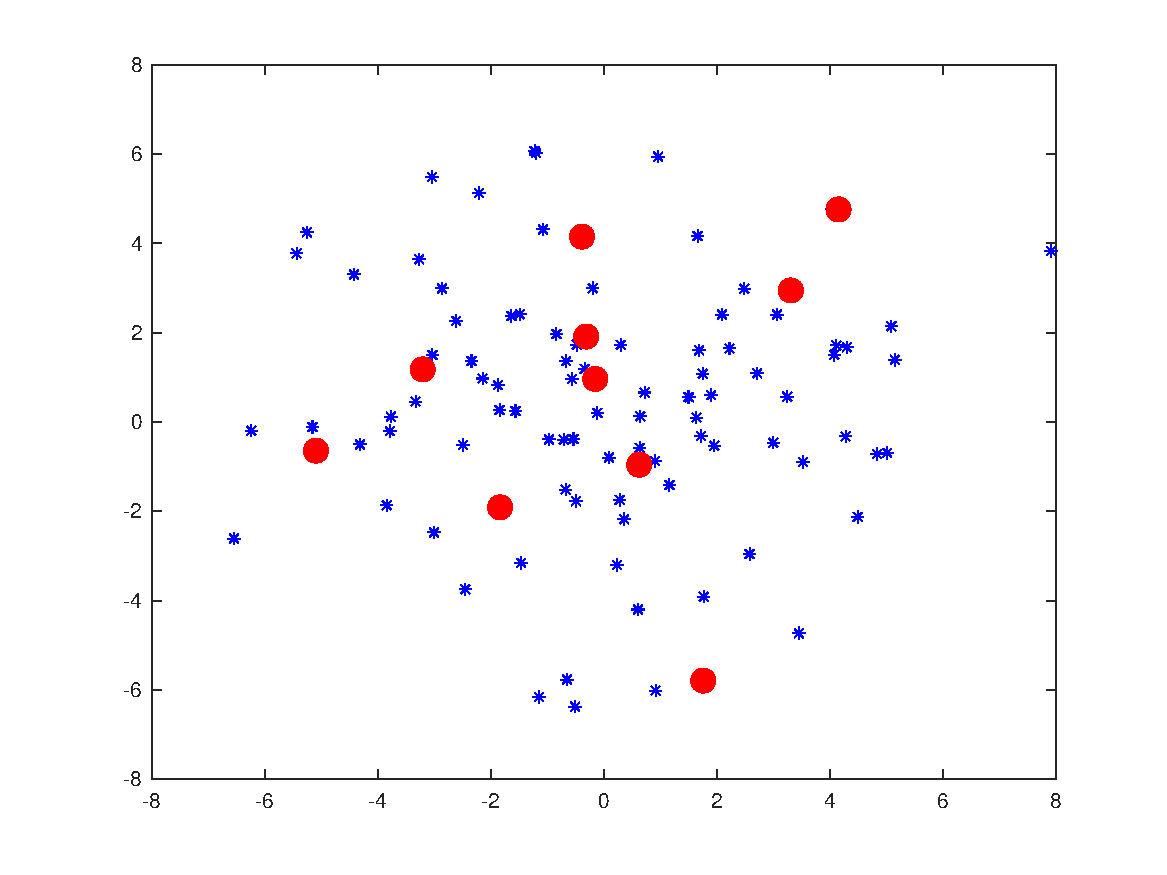
\includegraphics[width=\linewidth]{../src/figures/fixedsize/fixedsize_1}
    \caption*{$\sigma^2=0.01$}
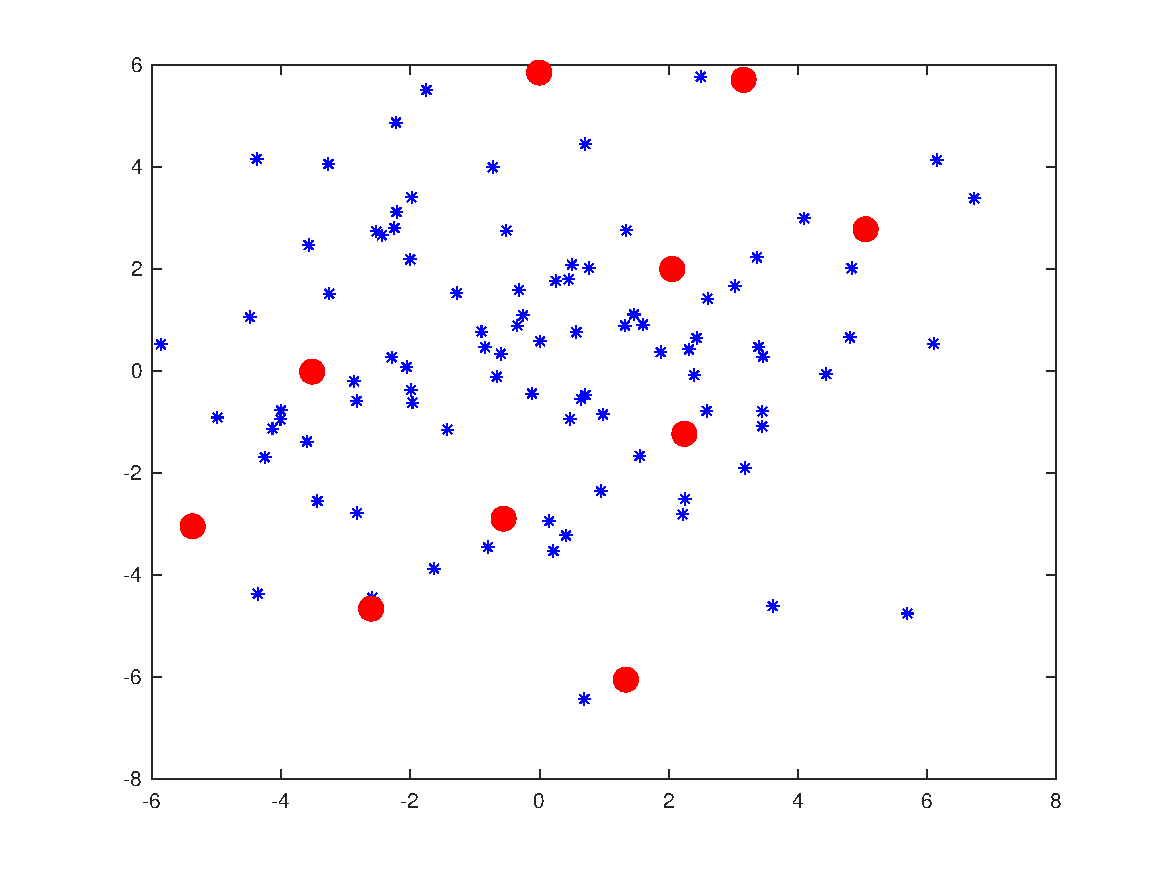
\includegraphics[width=\linewidth]{../src/figures/fixedsize/fixedsize_10}
    \caption*{$\sigma^2=0.1$}
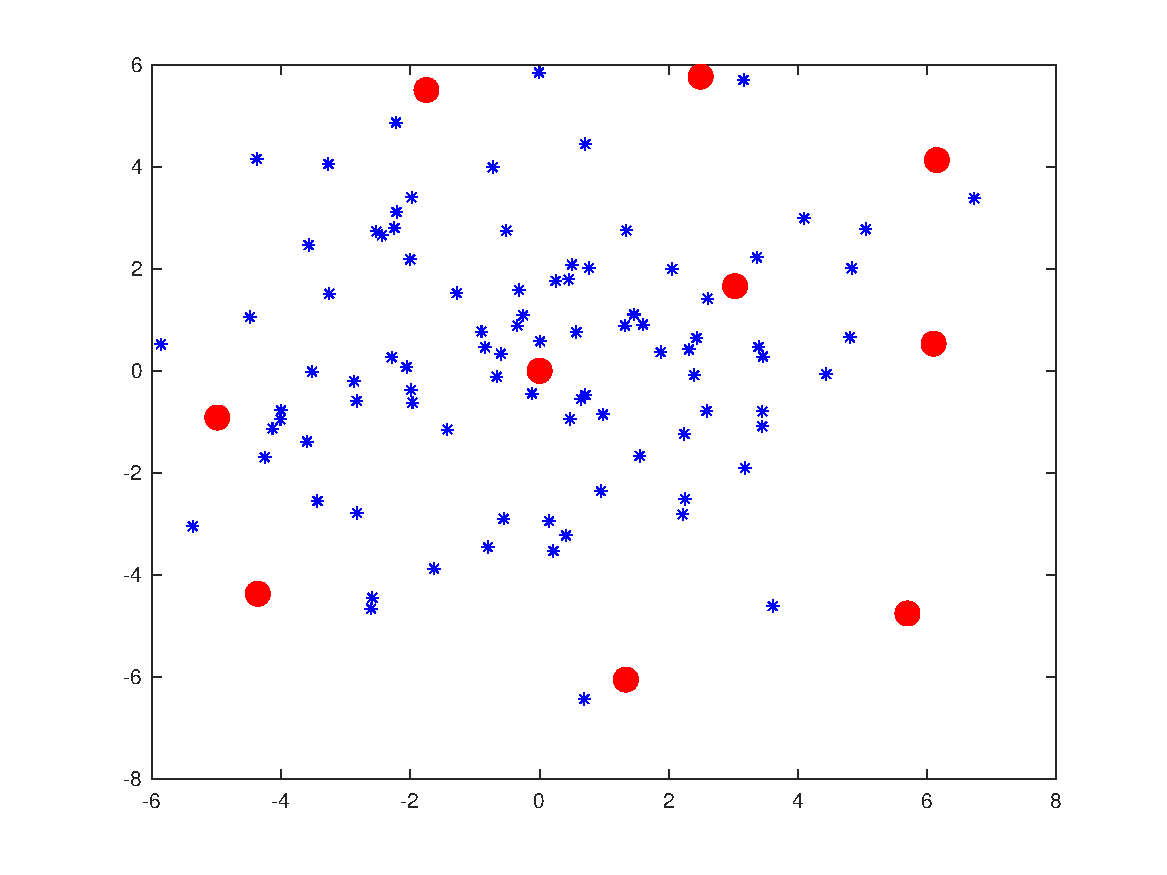
\includegraphics[width=\linewidth]{../src/figures/fixedsize/fixedsize_100}
    \caption*{$\sigma^2=1.0$}
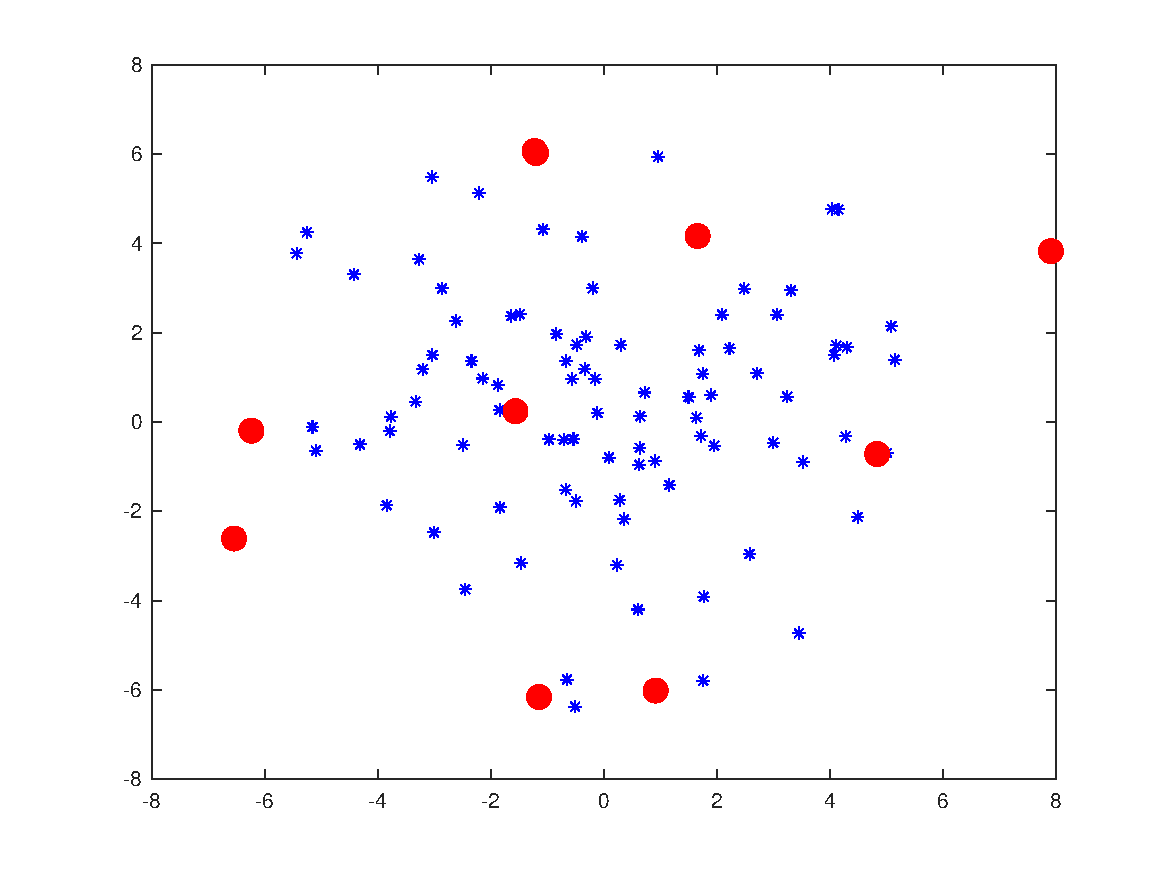
\includegraphics[width=\linewidth]{../src/figures/fixedsize/fixedsize_1000}
    \caption*{$\sigma^2=10.0$}
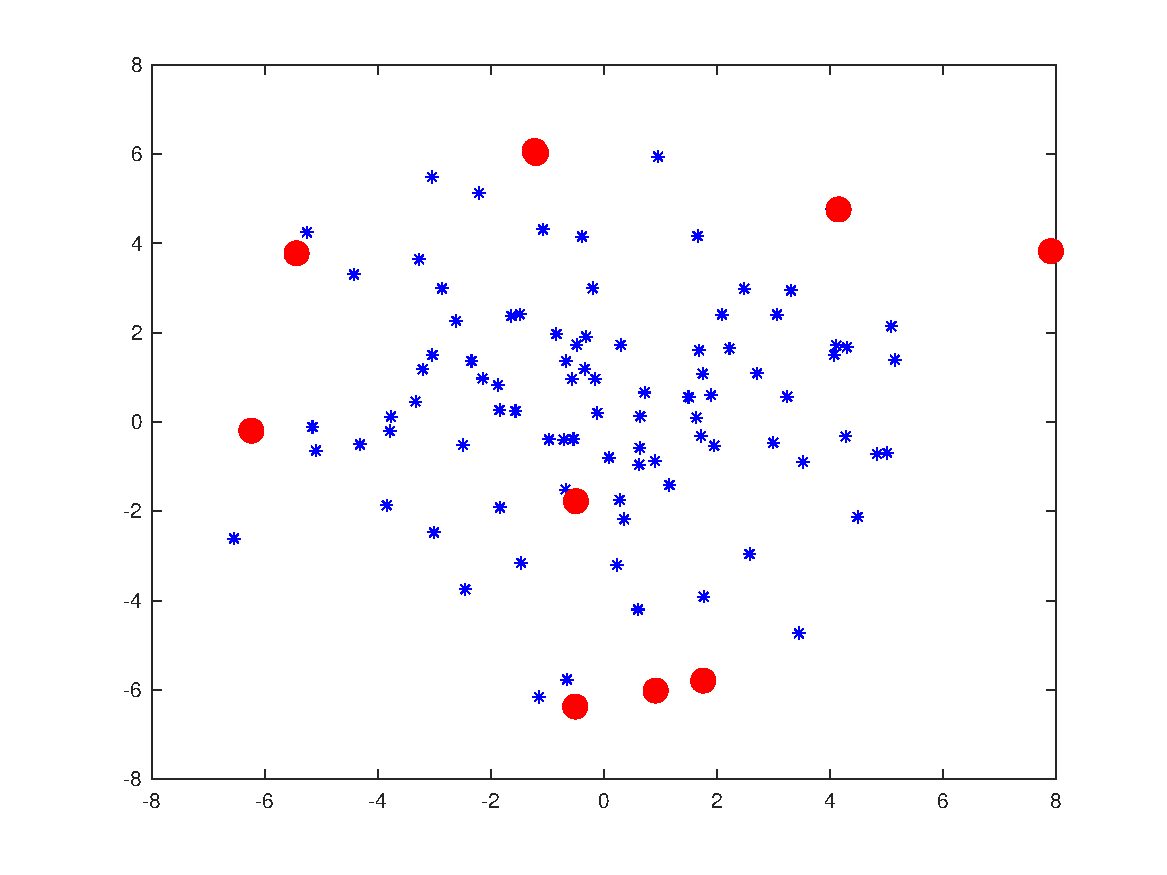
\includegraphics[width=\linewidth]{../src/figures/fixedsize/fixedsize_10000}
    \caption*{$\sigma^2=100.0$}
\end{minipage}
\caption{Subsample of input data points obtained for a fixed-sized LS-SVM using an RBF kernel of varying $\sigma^2$.}
\label{fixedsample}
\end{wrapfigure}

\par Experiments with an RBF kernel are shown in figure \ref{spectraltoy}. Since the similarity matrix is the Kernel function and $\sigma^2$ happens to control the contrast in similarity between data points a $\sigma^2$ value which is small leads to a single class as all points are considered similar while a larger $\sigma^2$ leads to poor clustering results.

\fakesubsection{Fixed-size LS-SVM}{}

Sometimes the amount of data that is being dealt with is too large such that some of the matrices like the kernel matrix involved in the dual formulations cannot be stored in memory. It becomes desirable, then, to solve the problem in the primal rather than in the dual space (it's the other way round when the number of input dimensions is high). The problem with this is that the feature map $\phi(x)$ is generally not known, only the kernel function representing dot products is made explicit.

\par While decomposition can be used for this an approach that can be considered in the case of fixed-size LS-SVMs is related to the Nystr\"om method which is traditionally used for integral approximation. In the current setting it means that one takes a set of support vectors of the input data (of size $M\ll N$) and then uses it to approximate the feature map $\phi(x)$ such that a parametric solution can be found. For fixed-size LS-SVMs the subsample starts randomly and is then updated iteratively as long as the Renyi entropy improves. This metric can be approximated by taking the sum of the elements of the kernel. This makes it fast to compute which is important in the context of big data (besides accuracy).

\par Examples of subsamples obtained through optimisation of the Renyi entropy are shown in figure \ref{fixedsample}. The kernel is a Gaussian one, the input data is normally distributed. It looks as though a larger value for $\sigma^2$ leads to a selection of data points that are more spread out. This is normal ; maximising the entropy means that one maximises the uncertainty, diversity or un-informativeness of the system. As the bandwidth increases the reach of each data point gets larger, the similarity with distant points increases and maximising entropy - which involves prioritisation of dissimilar points - causes points maximally distantiated from each other to be picked as support vectors.

\par In figure \ref{fscomp} a fixed-size LS-SVM approach is compared with a variant which applies an $\ell_0$-penalty after generating a fixed-size LS-SVM solution. The goal is to increase sparsity as determining $M$ isn't trivial. The post-processing does not influence the total runtime because its complexity is $\mathcal{O}(M^3)$ while that of the fixed-size LS-SVM is $\mathcal{O}(NM^2)$. While the error increases the number of support vector is much lower for the latter method. This is not surprising since the $\ell_0$-norm counts the number of non-zero values which means that it aims for sparse representations. It may not be the most sparse representation possible ; as obtaining $ell_0$ is NP-hard only a local minimum is found through an iterative procedure. The error for the post-processed LS-SVM drops as well, presumably because the model generalises better.

\fakesubsection{Kernel principal component analysis}{}

De-noising a quite noisy USPS dataset with classical PCA gives poor results at best (see figure \ref{usps_linear}). Kernel PCA with an RBF kernel manages to exploit the data much more and the results are a big improvement (see figure \ref{usps_kernel}).

\endgroup

What was noted in the yin-yang toy dataset shown at the beginning of this section can be observed again in figure \ref{uspsband} ; small bandwidths remove important information (such that some digits get reconstructed without noise but as the wrong number) while larger ones fail to de-noise and noise is re-introduced slowly but surely in the reconstructions. Eventually the results resemble that of classical, linear PCA.

\par The small bandwidths cause the data points to be considered highly dissimilar and directions of largest variation do not correspond to clusters with the same digits - rather, every data point is its own little cluster and variation is large in many meaningless directions. Conversely, very high bandwidths cause the data points to be considered very similar to each other and it once again gets hard to find meaningful directions of variation such that noise shared by the data points may be considered informative again.

\begin{figure}[h]
\centering
%
\subfloat[Error estimation.]{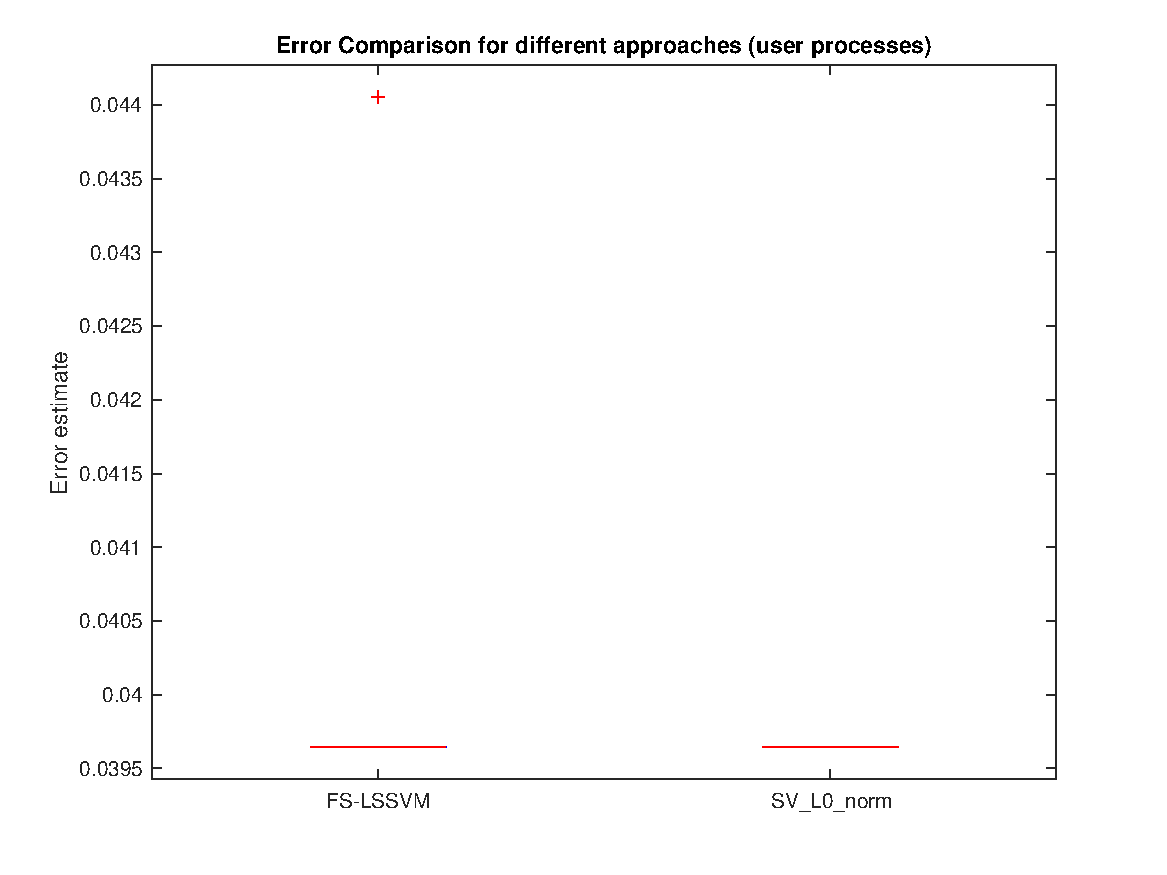
\includegraphics[width=0.25\textwidth]{../src/figures/fixedsize/comparison_error}}\quad
\subfloat[Number of support vectors.]{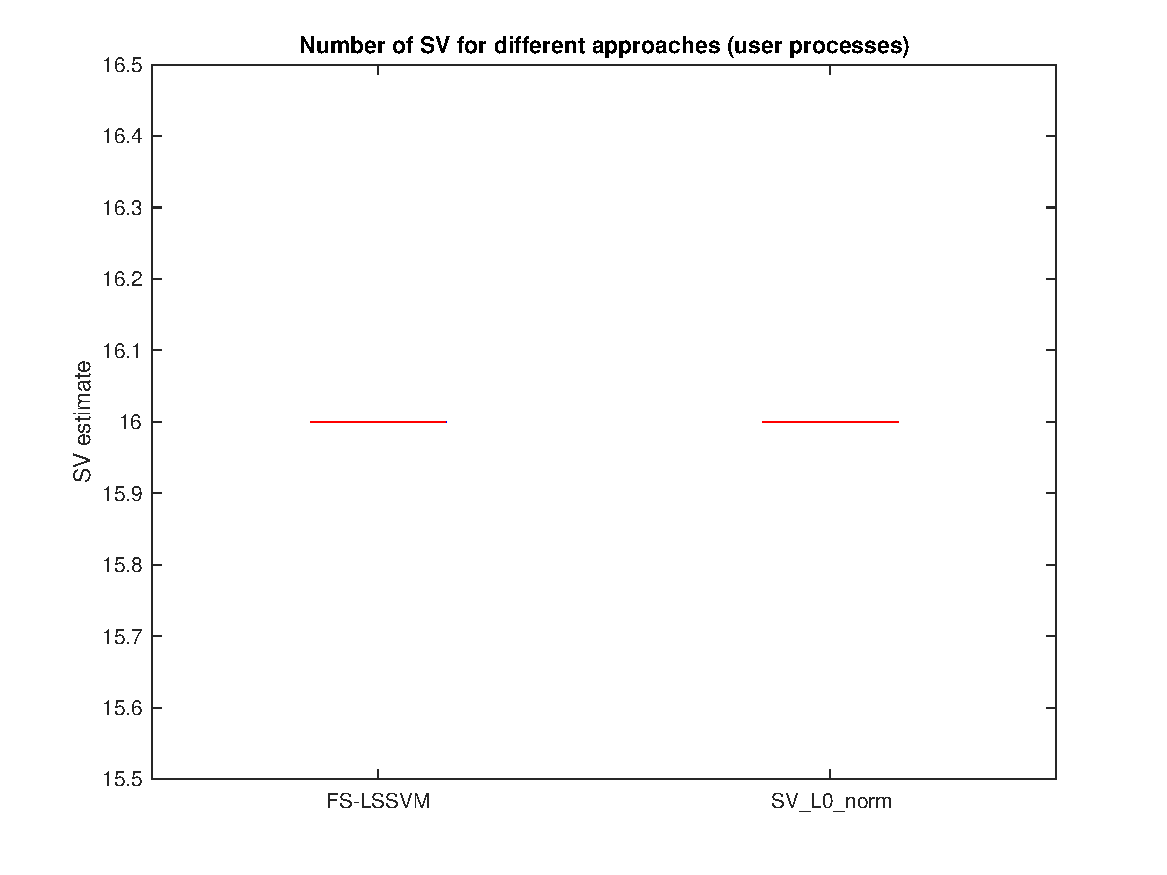
\includegraphics[width=0.25\textwidth]{../src/figures/fixedsize/comparison_sv}}\quad
\subfloat[Time taken for generating the models.]{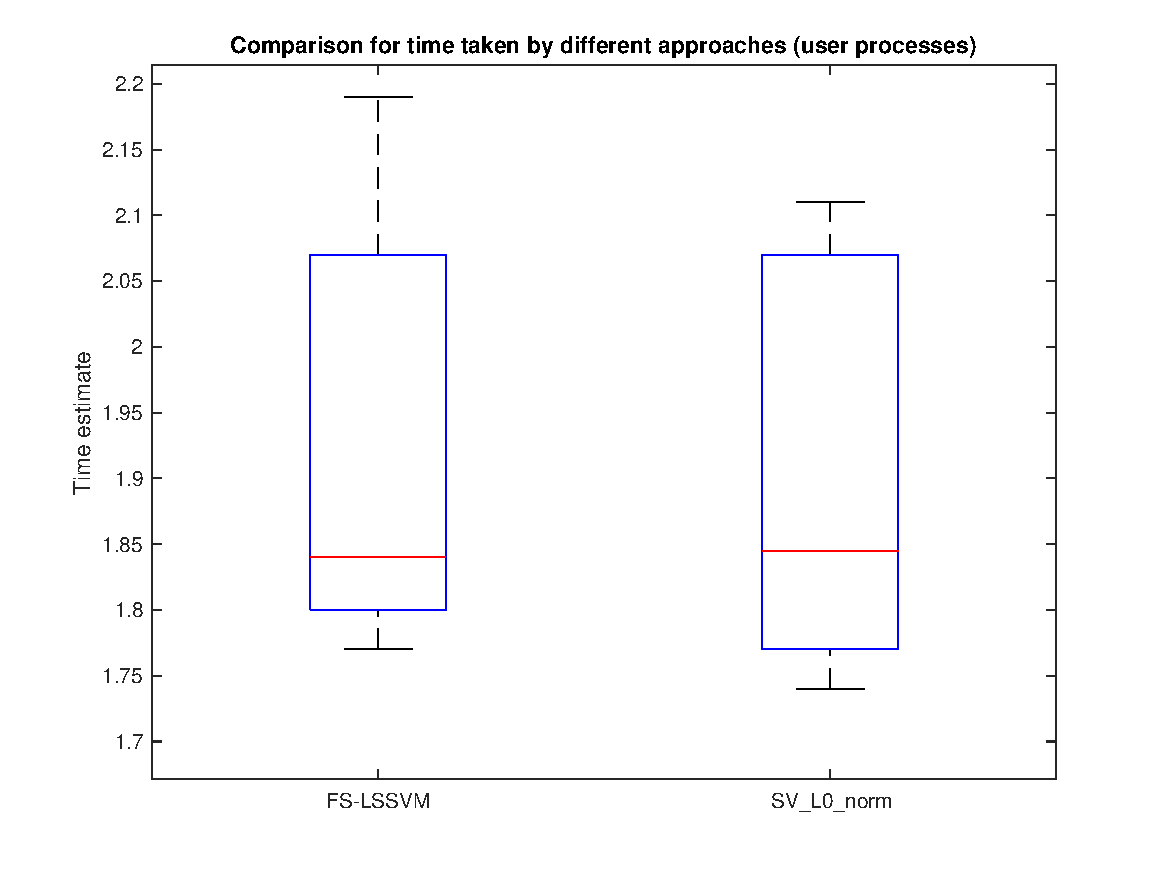
\includegraphics[width=0.25\textwidth]{../src/figures/fixedsize/comparison_time}}\\
%
\caption{Comparison of the standard fixed-size LS-SVM approach with a modified approach applying an $\ell_0$-penalty to obtain a sparser representation.}
\label{fscomp}
\end{figure}

\begin{figure}[h]
    \centering
    \begin{minipage}{0.45\textwidth}
        \centering
        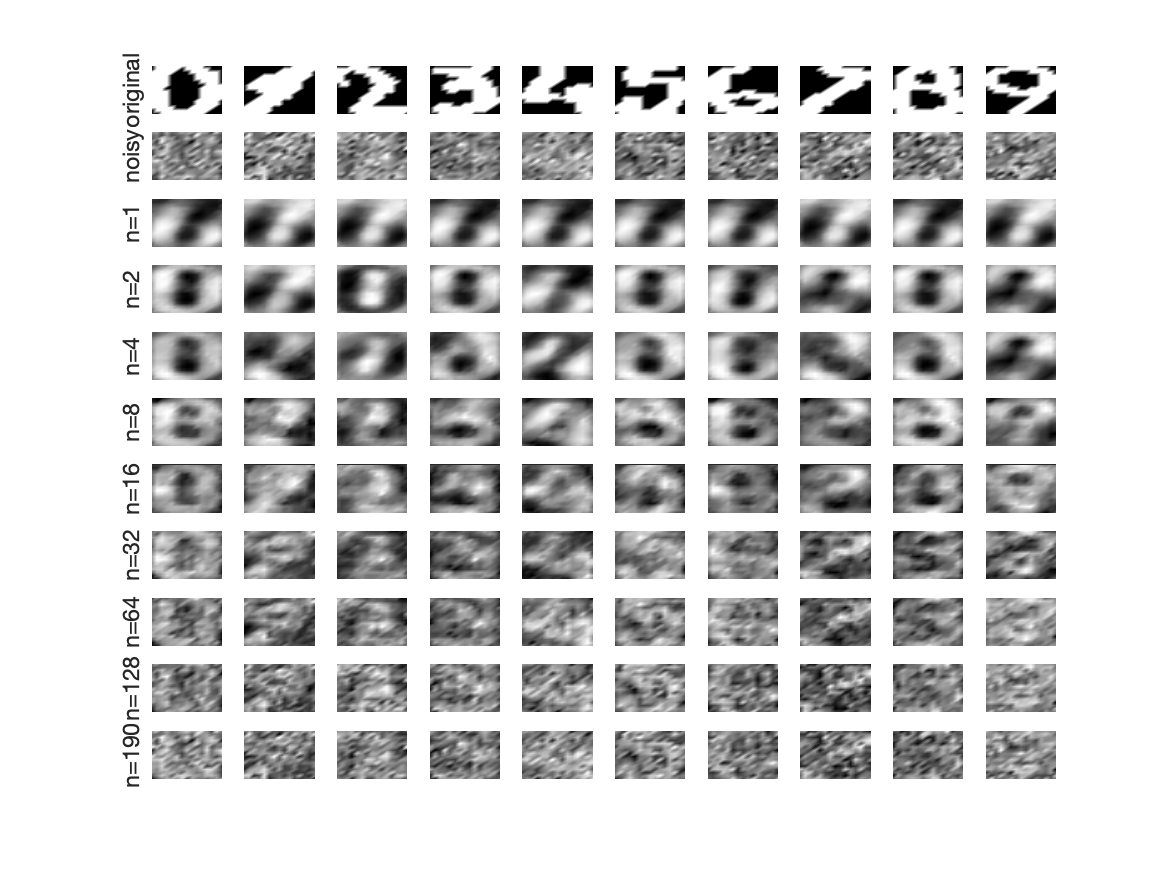
\includegraphics[width=1\textwidth]{../src/figures/usps/linear_pca}
        \caption{Results of linear PCA applied to the USPS dataset (top rows are original and noisy data, next 9 rows are results for $n_c\in [1,2,4,8,16,32,64,128,190]$).}
\label{usps_linear}
    \end{minipage}\hfill
    \begin{minipage}{0.45\textwidth}
        \centering
        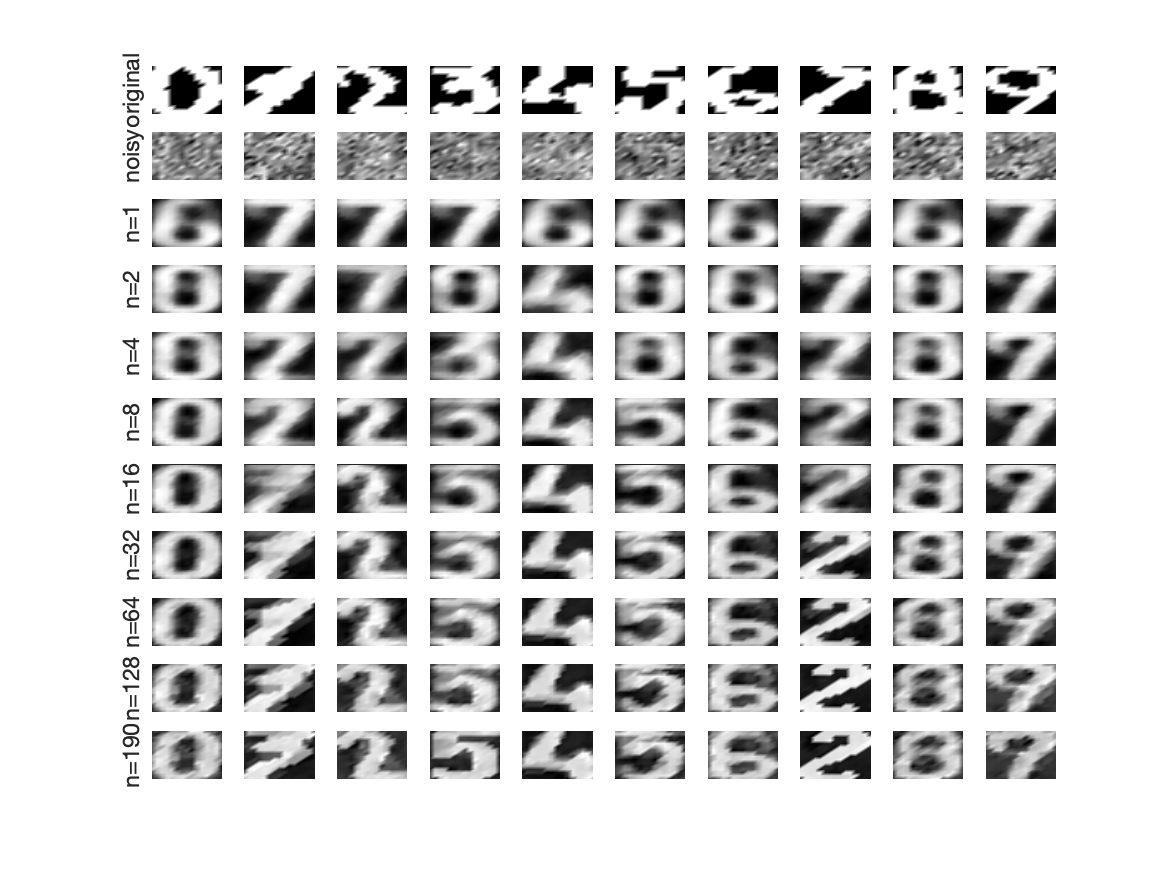
\includegraphics[width=1\textwidth]{../src/figures/usps/kernel_pca}
        \caption{Results of kernel PCA applied to the USPS dataset (top rows are original and noisy data, next 9 rows are results for $n_c\in [1,2,4,8,16,32,64,128,190]$).}
\label{usps_kernel}
    \end{minipage}
\end{figure}

\par Of note ; for slightly too small bandwidths, say $f=0.01$ or $f=0.1$ it looks like reconstructions are simply training data samples. This appears to be caused by the algorithm that calculates pre-images. It's a fixed-point iteration algorithm that takes a linear combination of the training data at each step.

\begin{figure}[h]
\centering
%
\subfloat[$f=0.01$.]{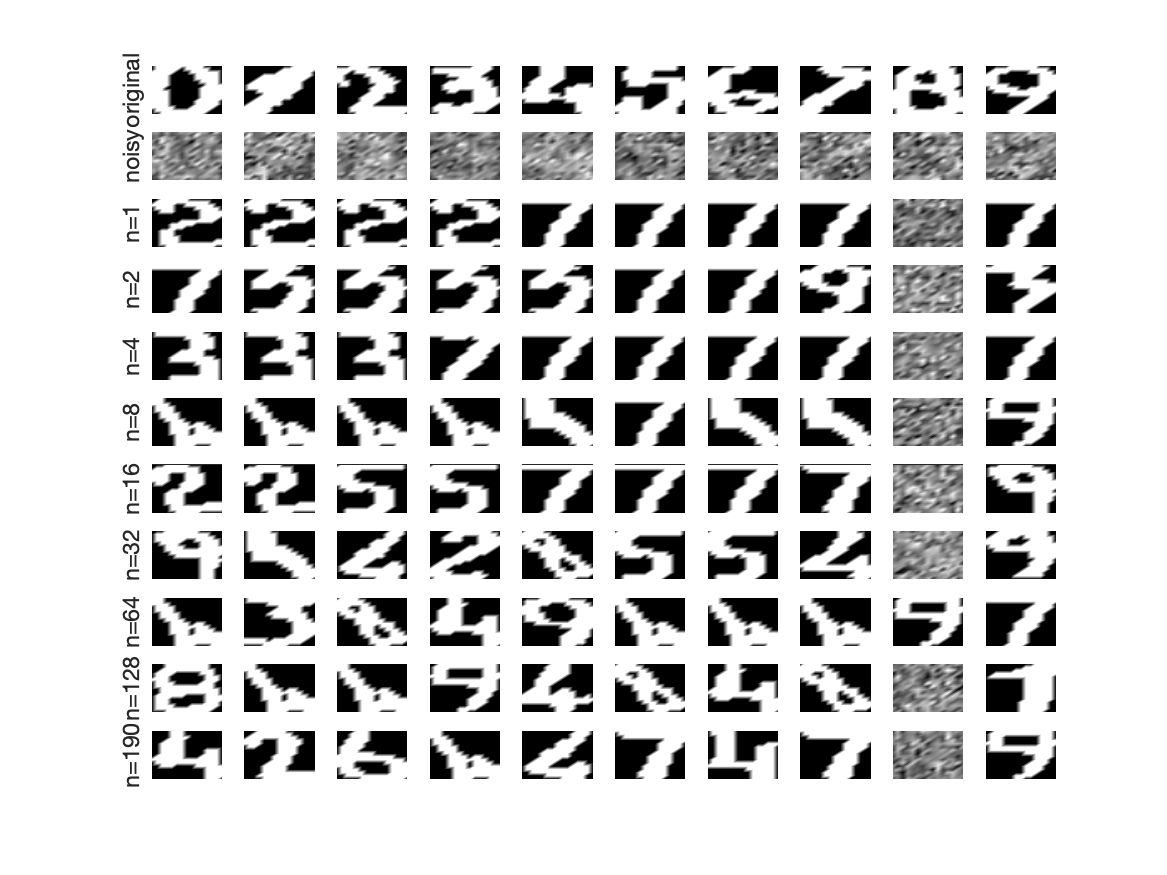
\includegraphics[width=0.25\textwidth]{../src/figures/usps/kernel_pca_001}}\hfil
\subfloat[$f=0.1$.]{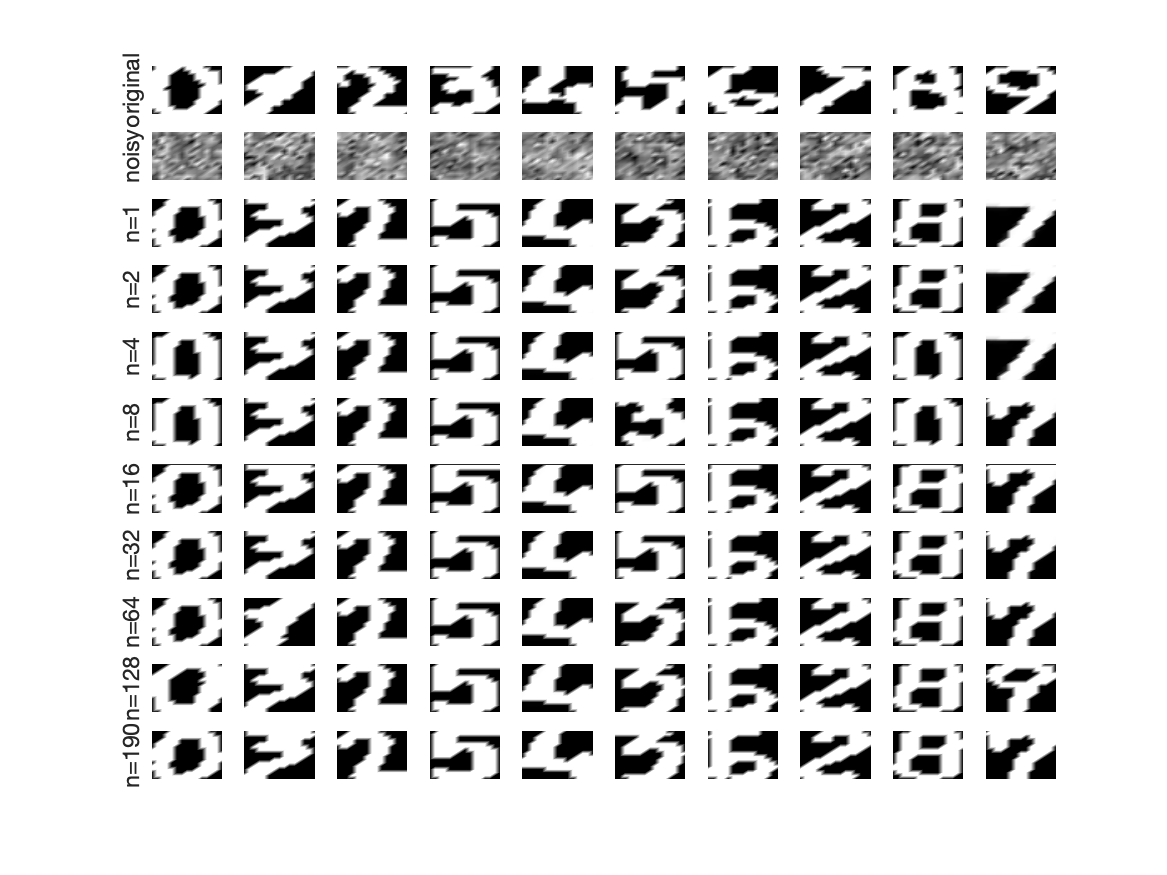
\includegraphics[width=0.25\textwidth]{../src/figures/usps/kernel_pca_01}}\hfil
\subfloat[$f=1.0$.]{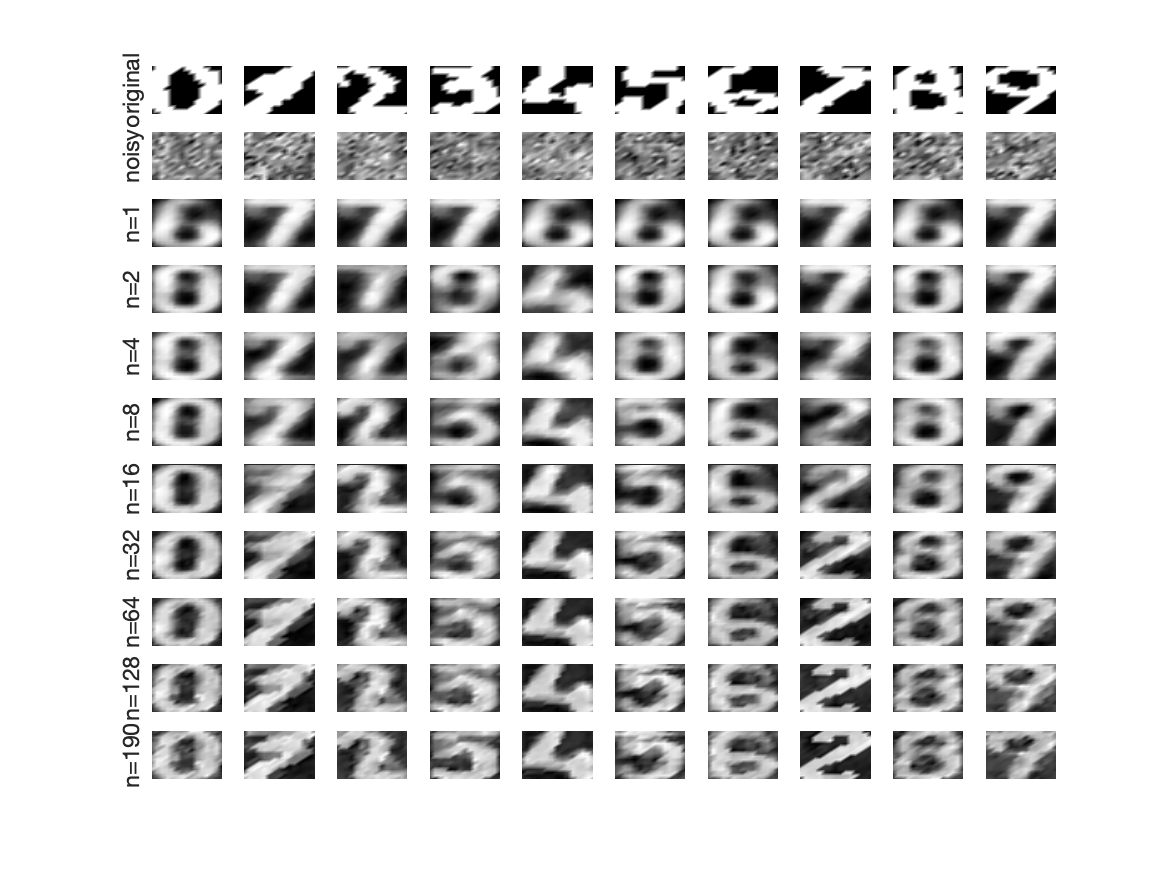
\includegraphics[width=0.25\textwidth]{../src/figures/usps/kernel_pca_1}}\hfil
\subfloat[$f=10.0$.]{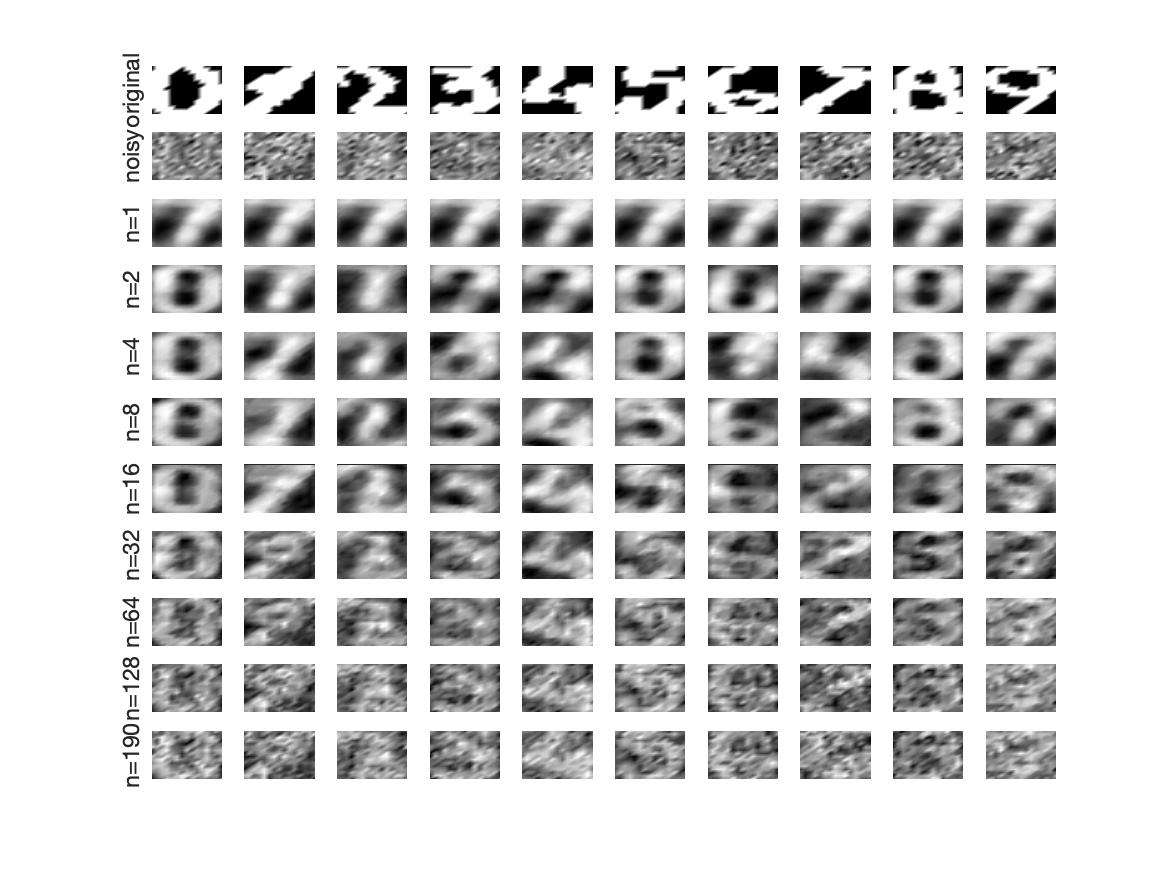
\includegraphics[width=0.25\textwidth]{../src/figures/usps/kernel_pca_10}}\\
%
%\subfloat[$f=100.0$.]{\includegraphics[width=0.30\textwidth]{../src/figures/usps/kernel_pca_5}}\quad
%\subfloat[$f=1000.0$.]{\includegraphics[width=0.30\textwidth]{../src/figures/usps/kernel_pca_6}}\quad
%\subfloat[$f=10000.0$.]{\includegraphics[width=0.30\textwidth]{../src/figures/usps/kernel_pca_7}}
%
\caption{De-noising the USPS hand-written digit dataset. $f$ is a factor with which is multiplied by about 51 to get the bandwidth. Very low and very high factors $f$ (e.g. 0.001 and 1000) lead to noisy reconstructions (resembling the second rows) and aren't pictured here.}
\label{uspsband}
\end{figure}

\par It was stated previously that one way to tune kPCA is to measure reconstruction errors for the validation set to gauge the effectiveness of certain parameter combinations. A plot of the reconstruction errors measured for the provided training and validation sets is shown in figure \ref{uspserror}. The errors tell a meaningful story which also corresponds to the visualisation of the performance of various parameter combinations in figure \ref{uspsband}.

\par Using the tuned parameters based on the contour plots better results are obtained. This can be seen in figure \ref{uspsresult}. The noise has been removed for the most part though one (and a half) de-noised digit is wrong.

\begin{figure}[h]
\centering
\subfloat[Results with linear PCA ($n_c=16$, first validation set) for comparison's sake.]{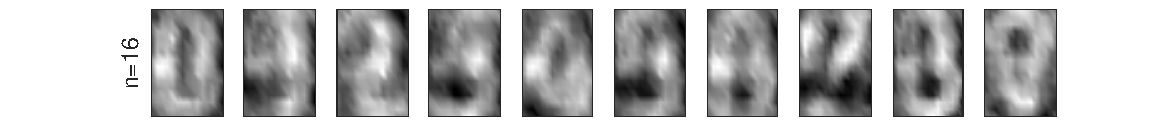
\includegraphics[width=0.7\linewidth]{../src/figures/usps/result_linear}}\hfil
\subfloat[Results for validation set 1.]{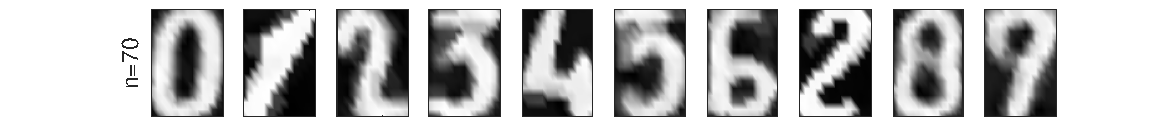
\includegraphics[width=0.7\linewidth]{../src/figures/usps/result_test1}}\hfil
\subfloat[Results for validation set 2.]{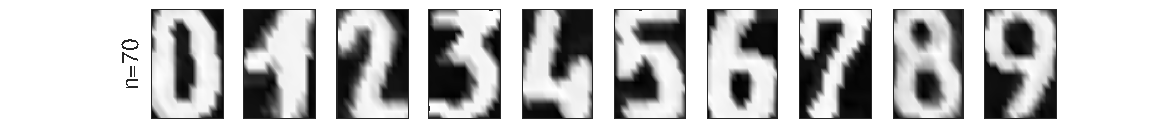
\includegraphics[width=0.7\linewidth]{../src/figures/usps/result_test2}}\hfil
\caption{Denoising of the USPS dataset using tuned parameters ($n_c=70,f=0.4$).}
\label{uspsresult}
\end{figure}

\begin{figure}[!htb]
\centering
\subfloat[Errors (root mean squared errors) for the training set.]{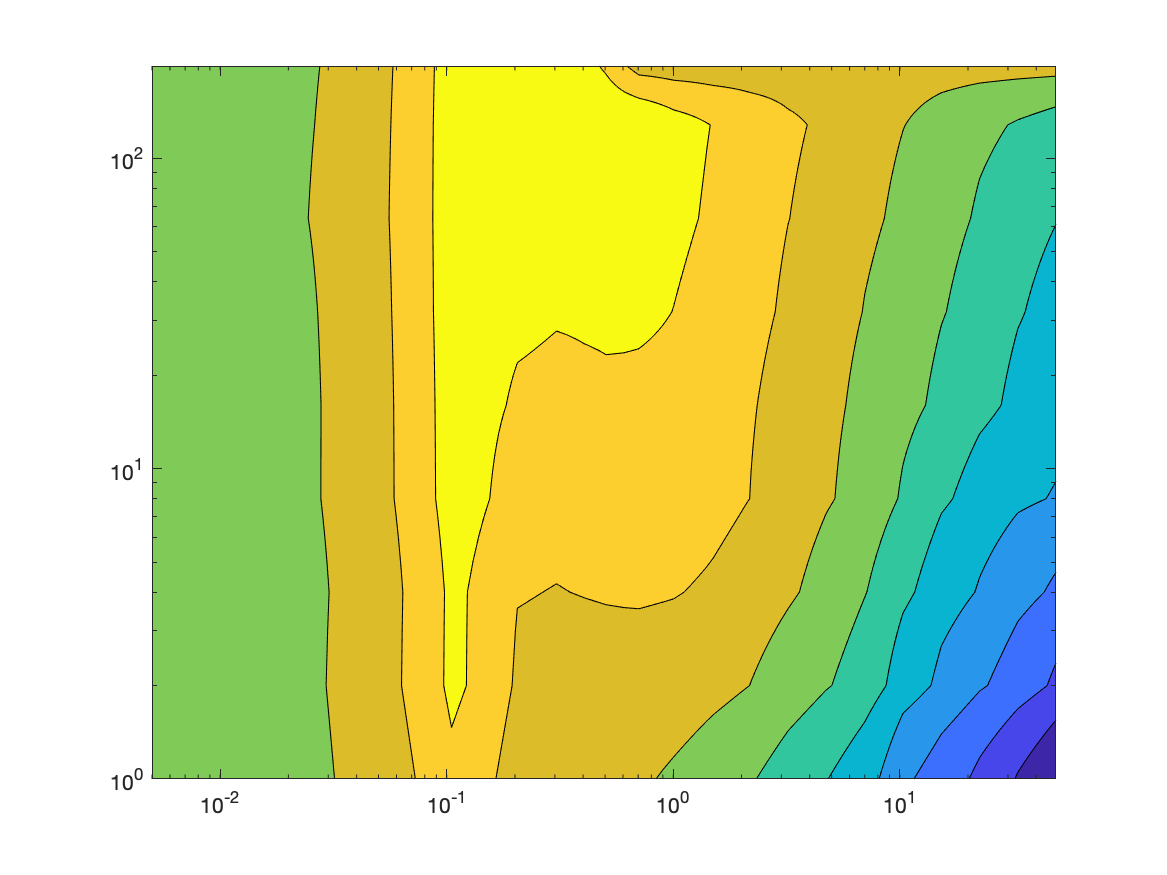
\includegraphics[width=0.32\textwidth]{../src/figures/usps/contour_xtrain}}\hfil
\subfloat[Errors (root mean squared errors) for the first test set.]{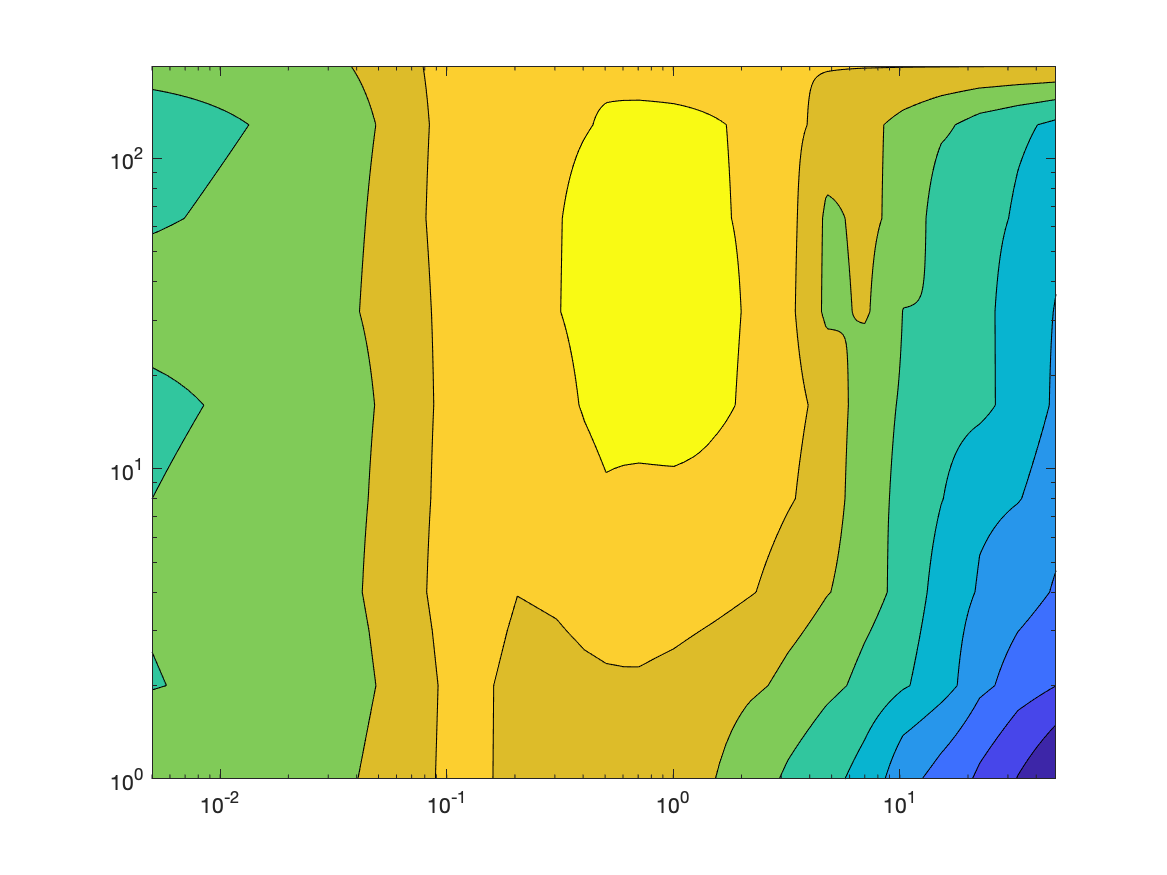
\includegraphics[width=0.32\textwidth]{../src/figures/usps/contour_xtest1}}\hfil
\subfloat[Errors (root mean squared errors) for the second test set.]{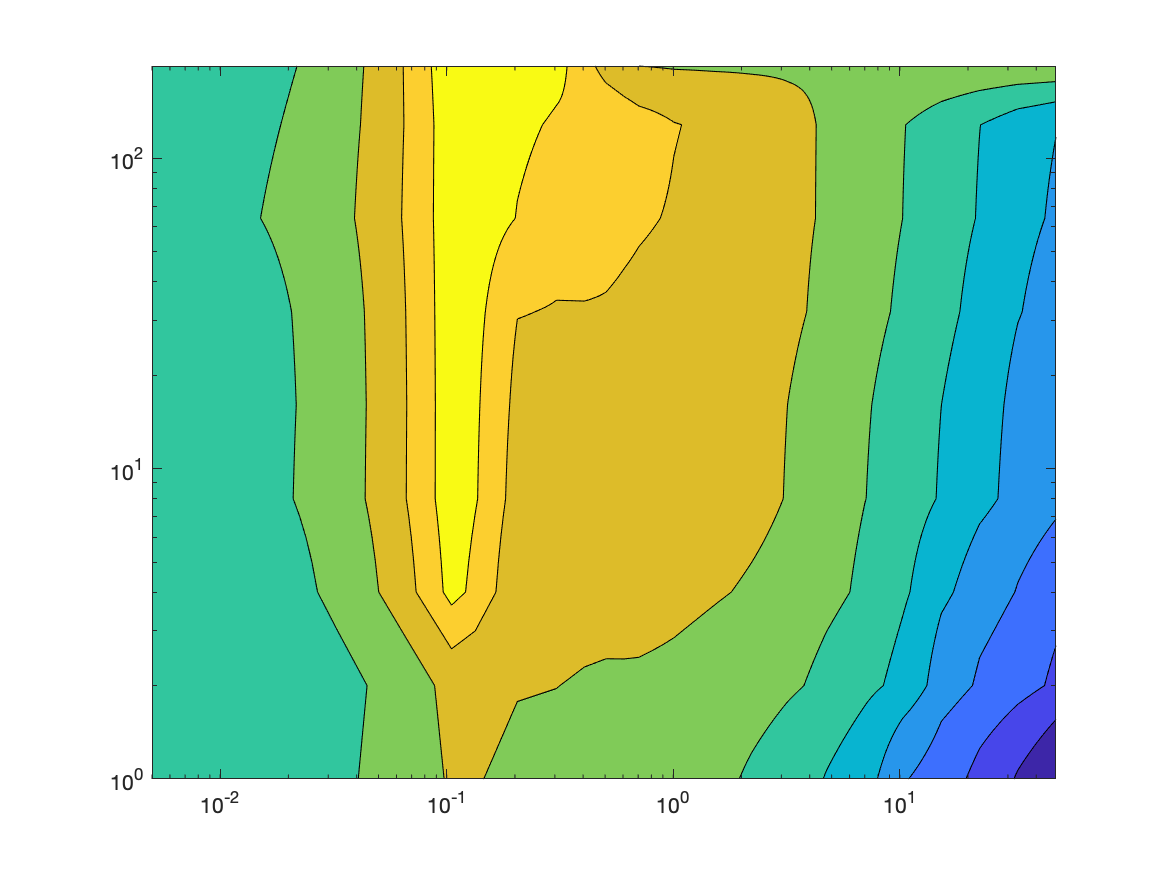
\includegraphics[width=0.32\textwidth]{../src/figures/usps/contour_xtest2}}\hfil
\caption{Reconstruction error for the training and validation sets in function of the bandwidth and the number of components. This is a crude grid search (x-axis represents the factor $f$, y-axis is the number of components) in combination with interpolation to construct a contour plot. The axes are scaled logarithmically. More appropriate tuning methods include kernel parallel analysis or Model selection based on Distance Distributions (MDD). As the number of components rises, the bandwidth can be higher before de-noising fails.}
\label{uspserror}
\end{figure}

\begin{figure}[h]
\centering
%
\subfloat[$\sigma^2=0.001$.]{
\begin{minipage}{0.48\textwidth}
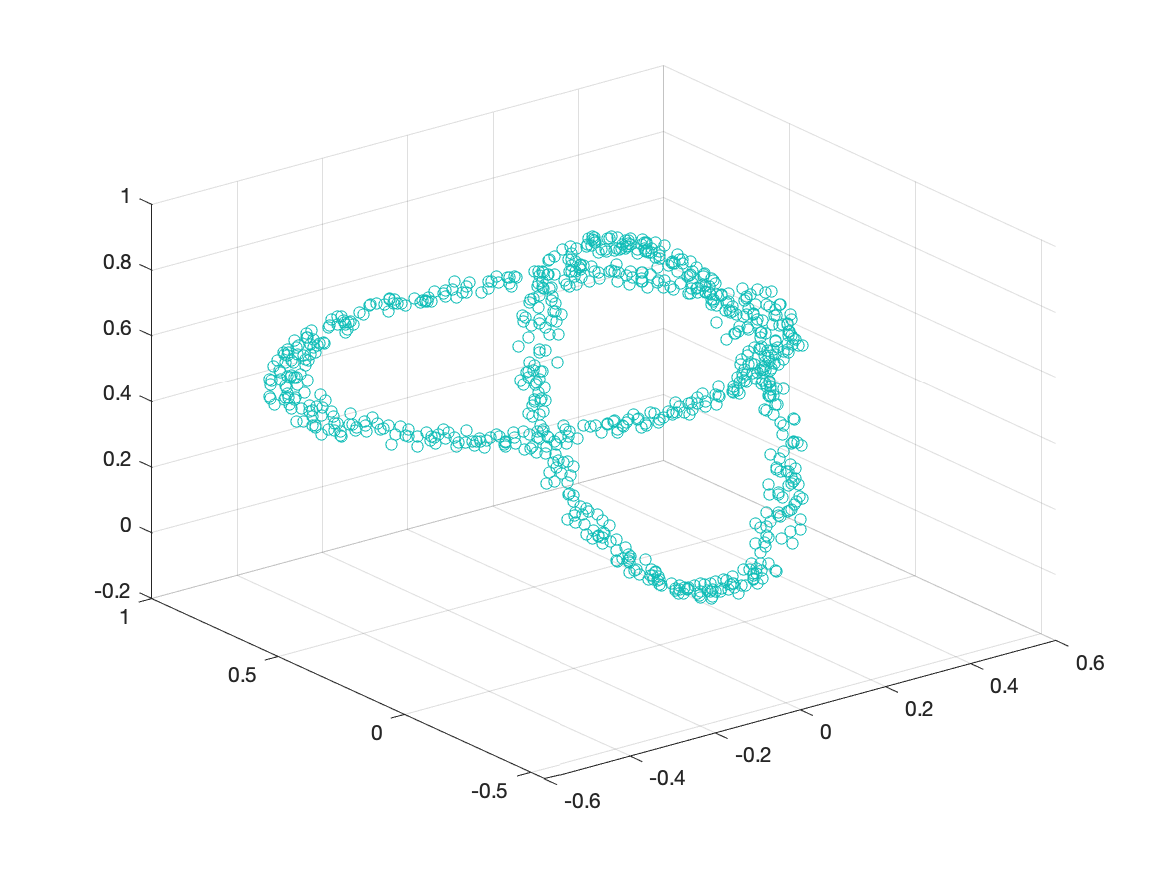
\includegraphics[width=0.45\textwidth]{../src/figures/spectral/rings_clusters_1}

\includegraphics[width=0.4\textwidth]{../src/figures/spectral/rings_block_1}
\end{minipage}}\quad
\subfloat[$\sigma^2=0.005$.]{
\begin{minipage}{0.48\textwidth}
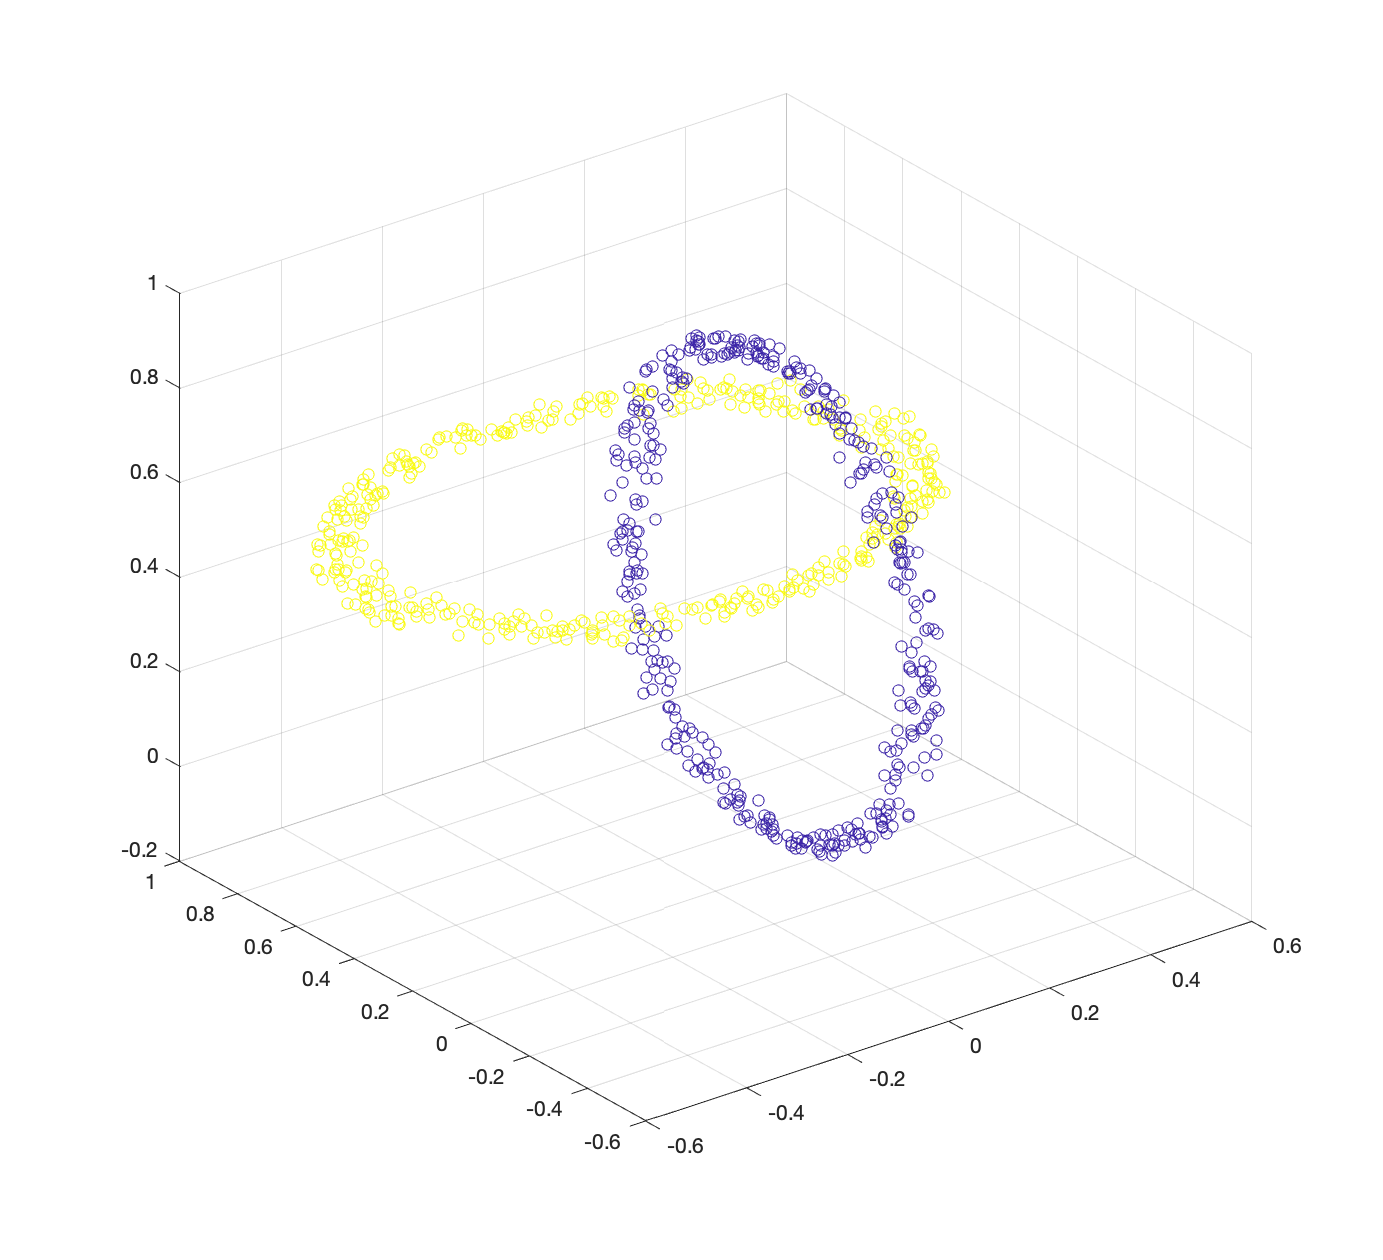
\includegraphics[width=0.45\textwidth]{../src/figures/spectral/rings_clusters_5}
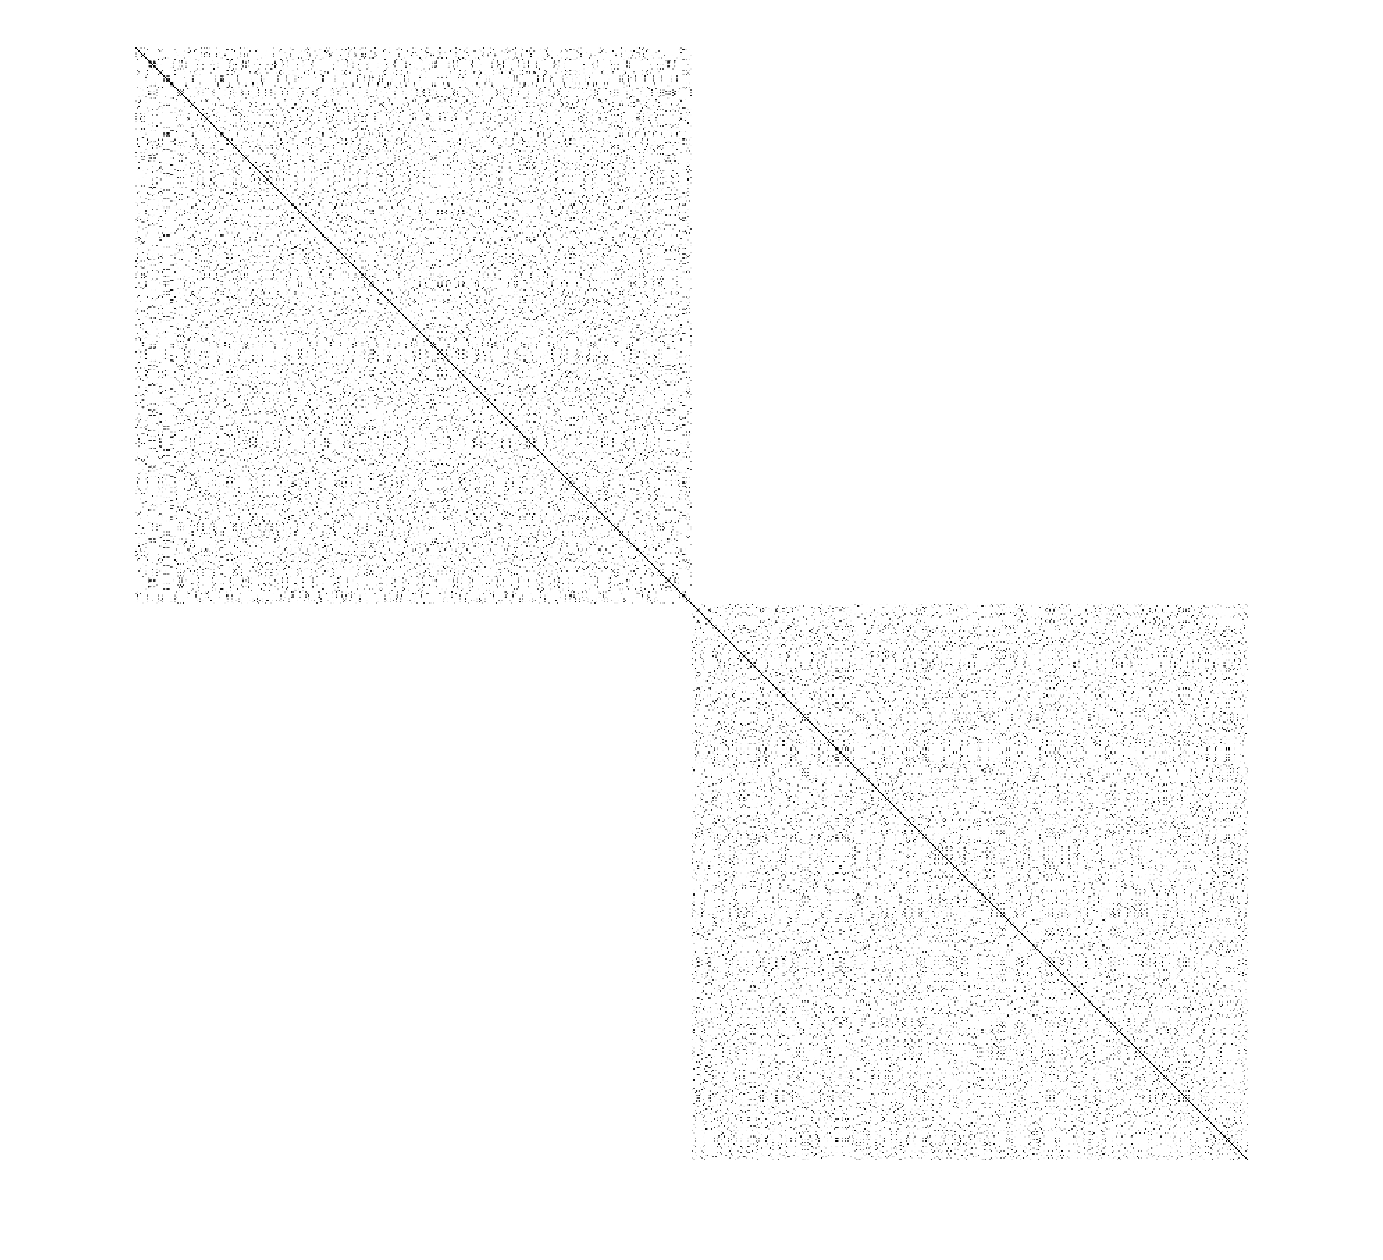
\includegraphics[width=0.4\textwidth]{../src/figures/spectral/rings_block_5}
\end{minipage}}\\
%
\subfloat[$\sigma^2=0.01$.]{
\begin{minipage}{0.48\textwidth}
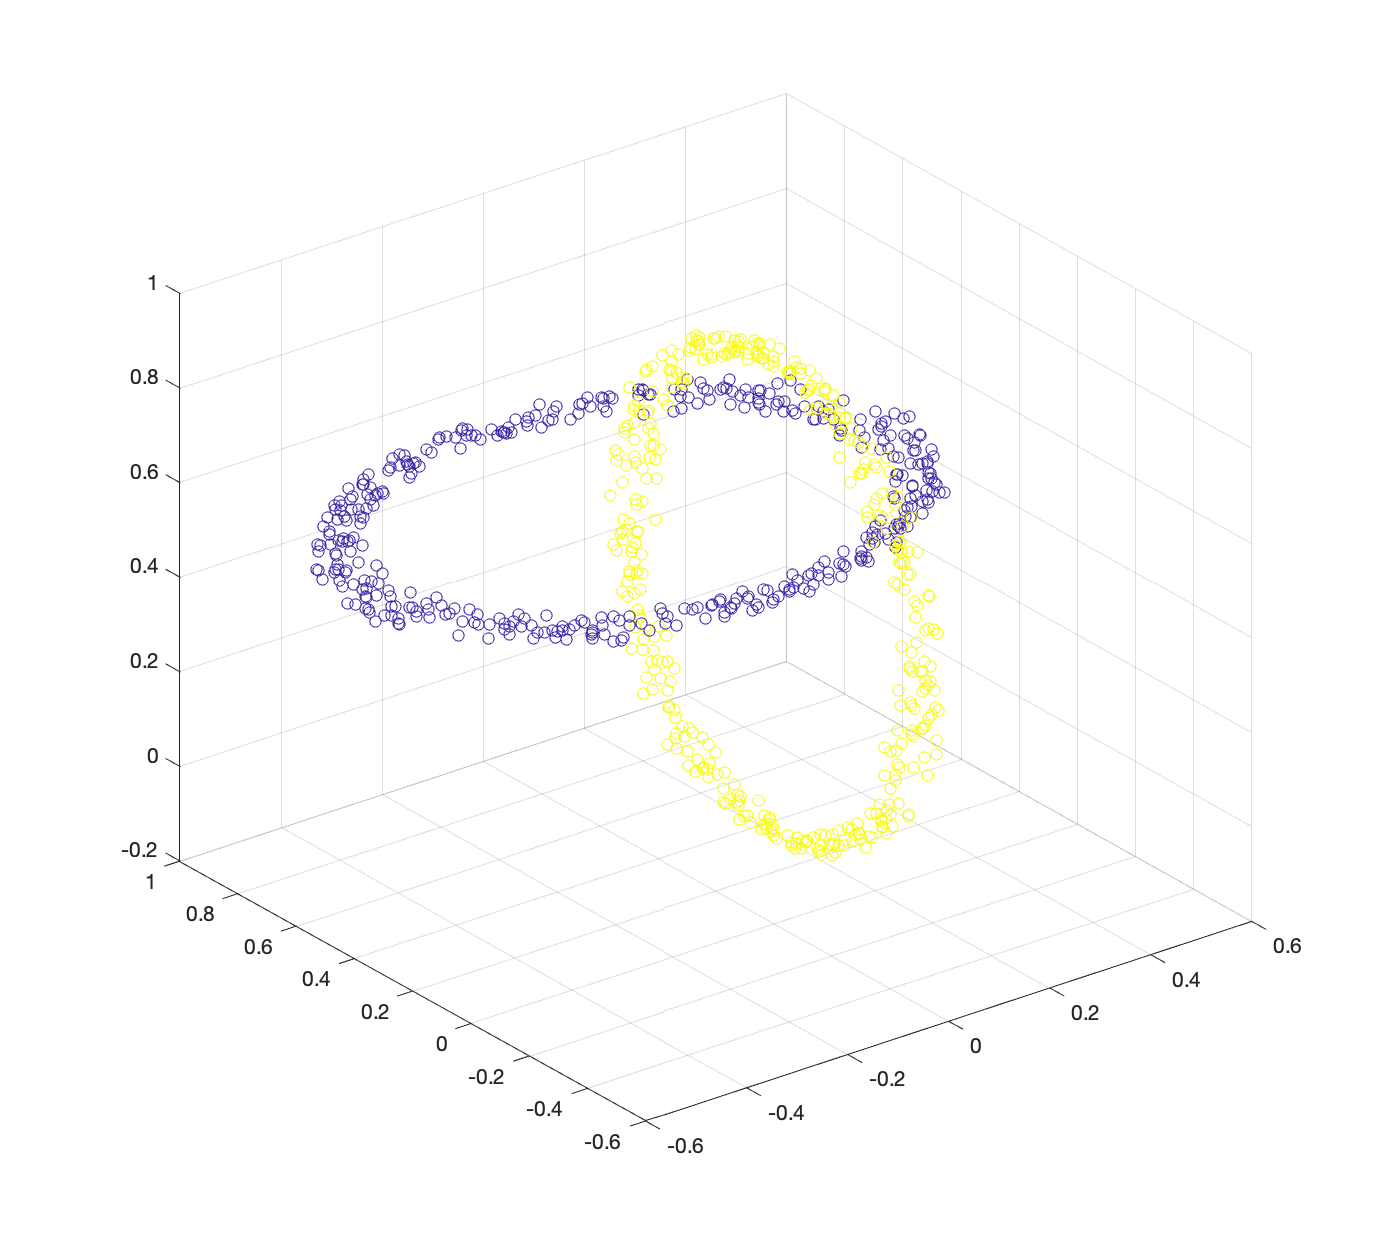
\includegraphics[width=0.45\textwidth]{../src/figures/spectral/rings_clusters_10}
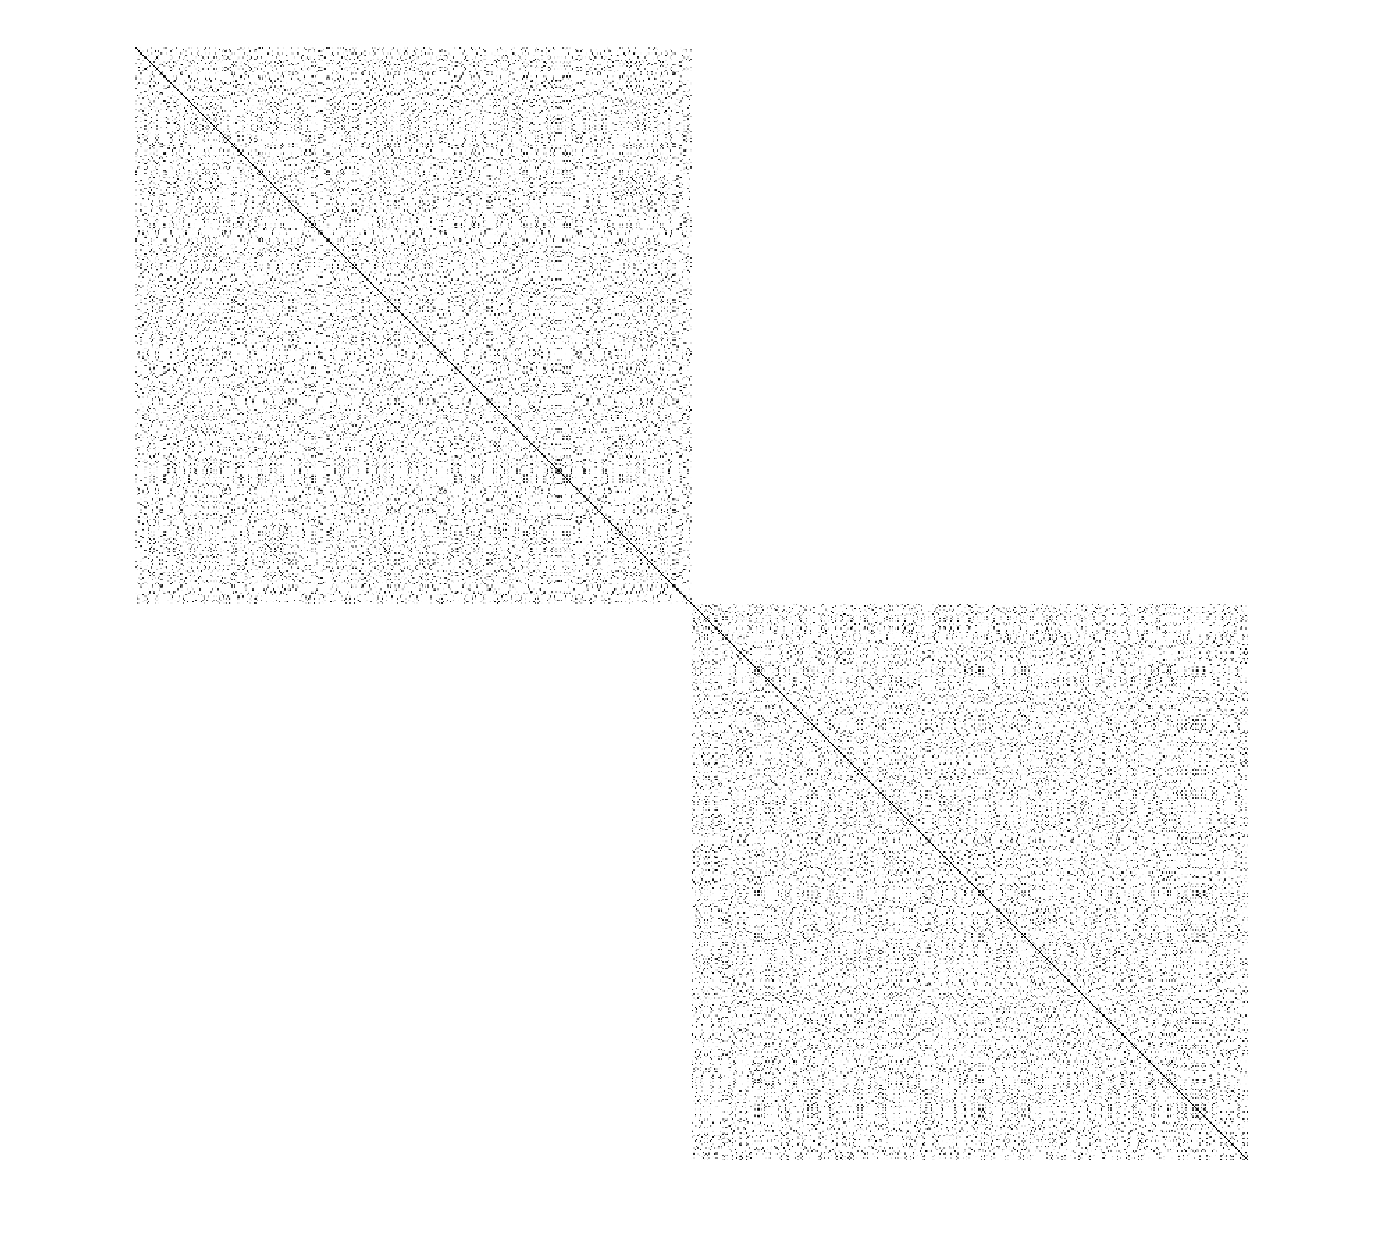
\includegraphics[width=0.4\textwidth]{../src/figures/spectral/rings_block_10}
\end{minipage}}\quad
\subfloat[$\sigma^2=1.0$.]{
\begin{minipage}{0.48\textwidth}
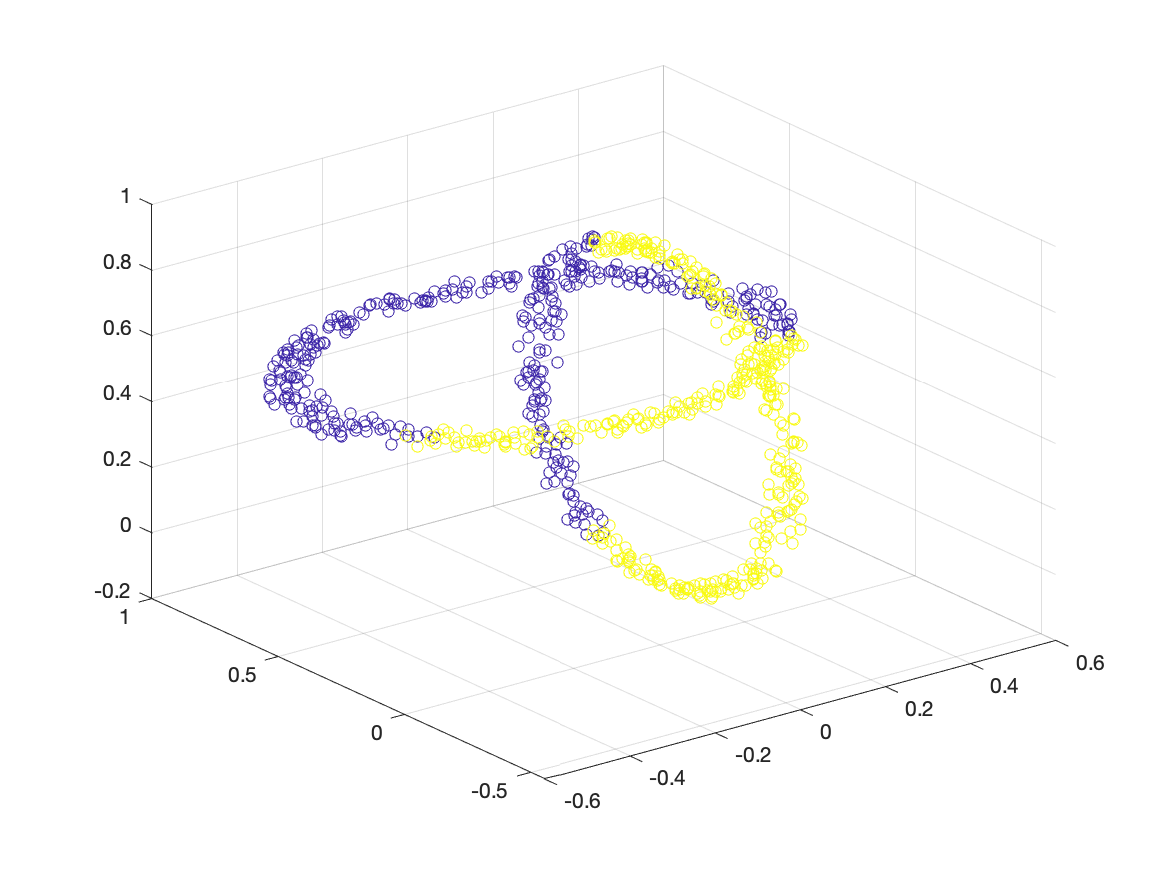
\includegraphics[width=0.45\textwidth]{../src/figures/spectral/rings_clusters_1000}
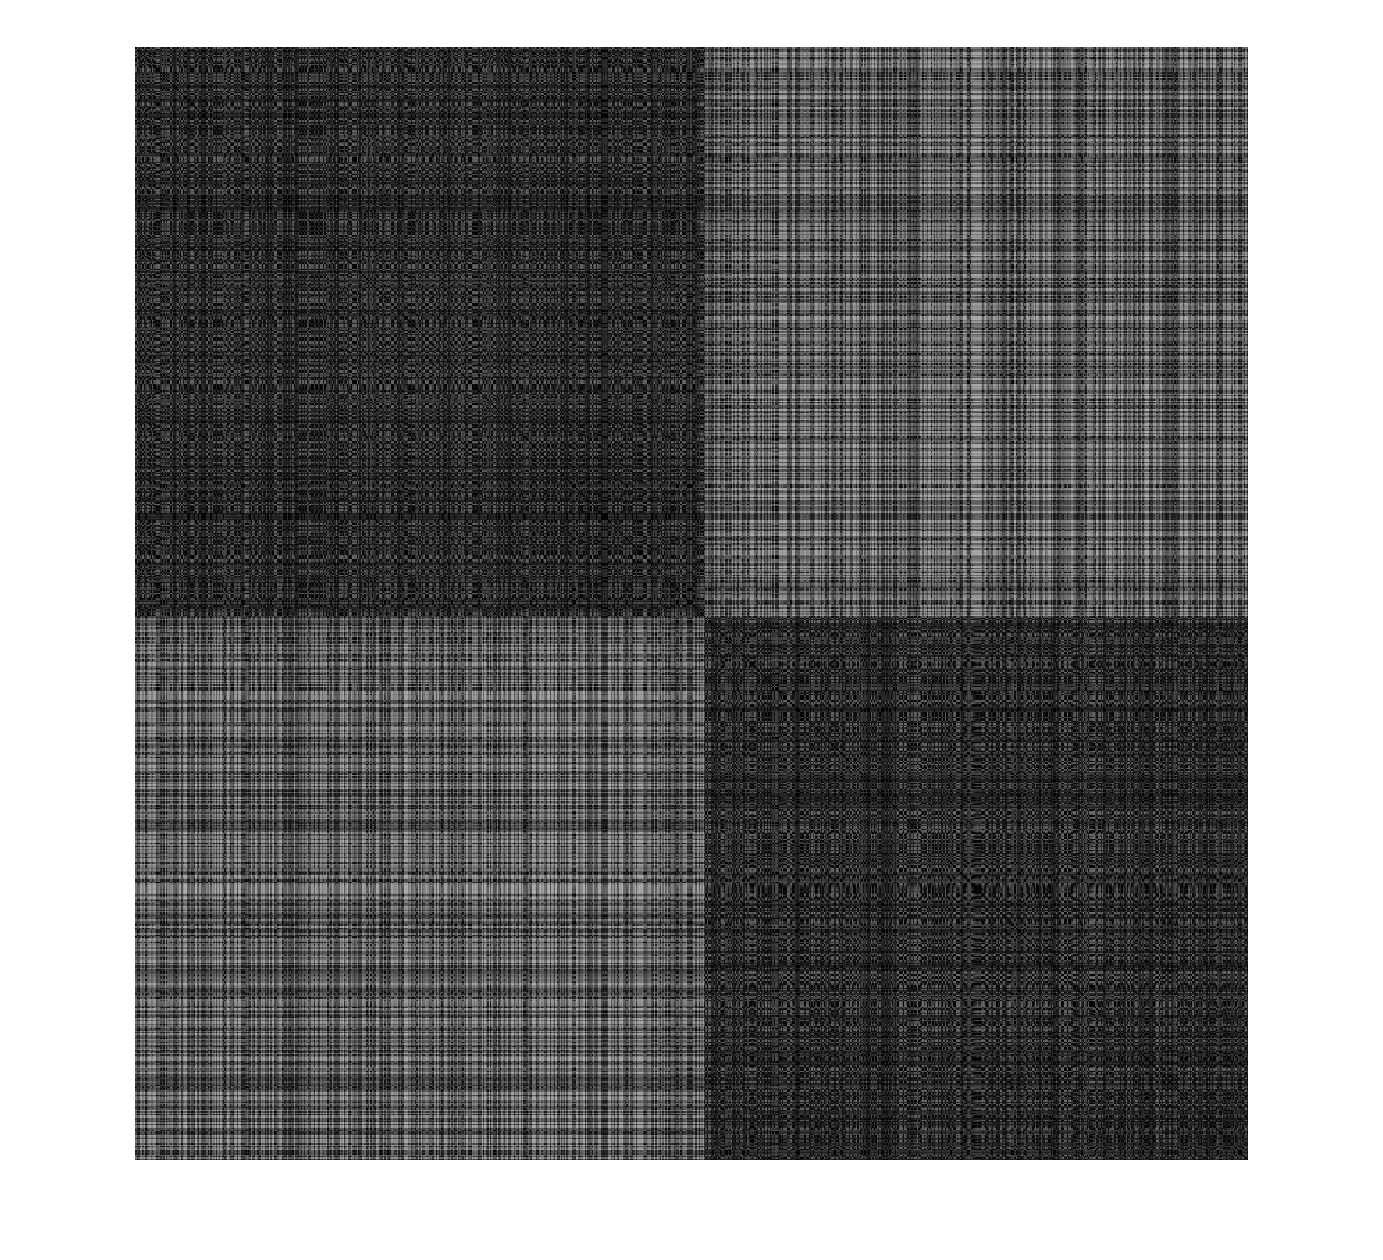
\includegraphics[width=0.4\textwidth]{../src/figures/spectral/rings_block_1000}
\end{minipage}}\\
%
\caption{Clustering of a toy dataset consisting of two rings. KSC applied using a kernel with varying $\sigma^2$ values. When this bandwidth is too large the reach of influence of each data point becomes too large and the clustering becomes subpar.}
\label{spectraltoy}
\end{figure}

\fakesubsection{Fixed-size LS-SVM}{}

Next, two datasets are experimented with. LS-SVM with or without sparisification is applied to the Shuttle - and then the California housing dataset. The first is a classification problem, the second a regression problem.

\fakesubsubsection{Shuttle dataset}{}

The Shuttle dataset has 58.000 train or test samples. It's a multi-class classification problem, having a total of 7 classes which are not equally represented. The first class represents 45.586 out of 58.000 samples or about $78.5\%$ of the dataset so generally 80\% is seen as the so-called majority rule and the aim is to reach an accuracy of at least 99\%. The class imbalance can be observed in the distributions (figure \ref{shuttlehist}).

\par The provided code reduces the dataset's size to 700 samples in which only 5 of the classes are present, presumably because of the long runtimes. It does not seem to handle multi-class problems per se but still makes use of the sign function for predictions effectively treating the problem as a one-versus-all problem. Therefore initial results see a fairly large error rate which tend to get even worse than the majority rule (especially when estimating the error based on the average across folds for 10-fold validation).

\par Instead of using the provided set, 3000 samples were picked (such that class 3 is represented more than once and stratification can be applied). Both a 80\%/20\% train/test split or only 10-fold cross-validation were experimented with for error estimation.

%\par For training, validation and evaluation a training set of 29.000 - and training and validation sets of both 14.500 samples were used (split randomly by stratification).

\begin{figure}[h]
\centering
%
\subfloat[First feature (time).]{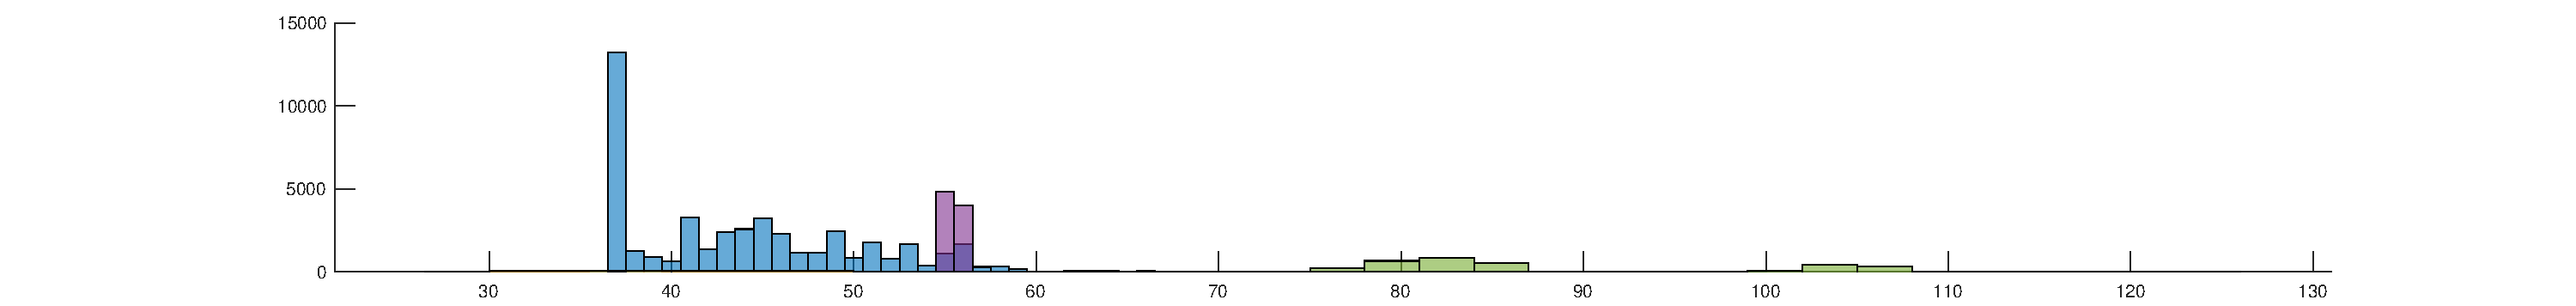
\includegraphics[width=\textwidth]{../src/figures/fssvm/shuttle_hist_1}}\\
\subfloat[First feature (time).]{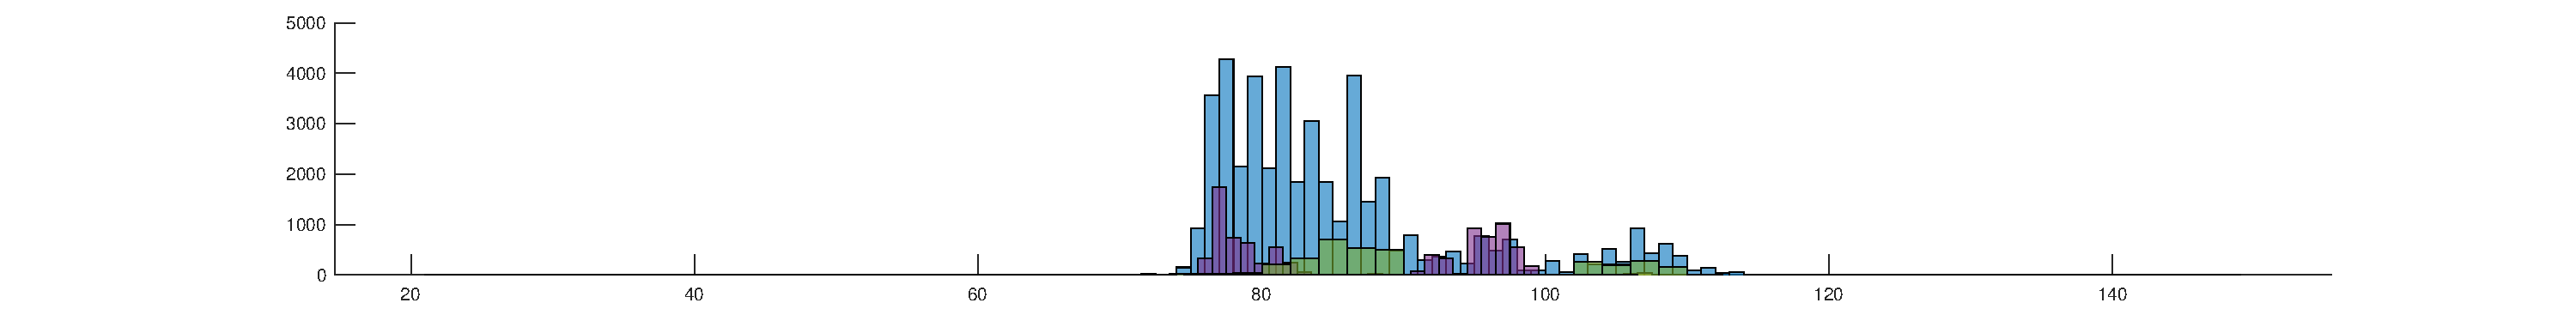
\includegraphics[width=\textwidth]{../src/figures/fssvm/shuttle_hist_3}}\\
\subfloat[First feature (time).]{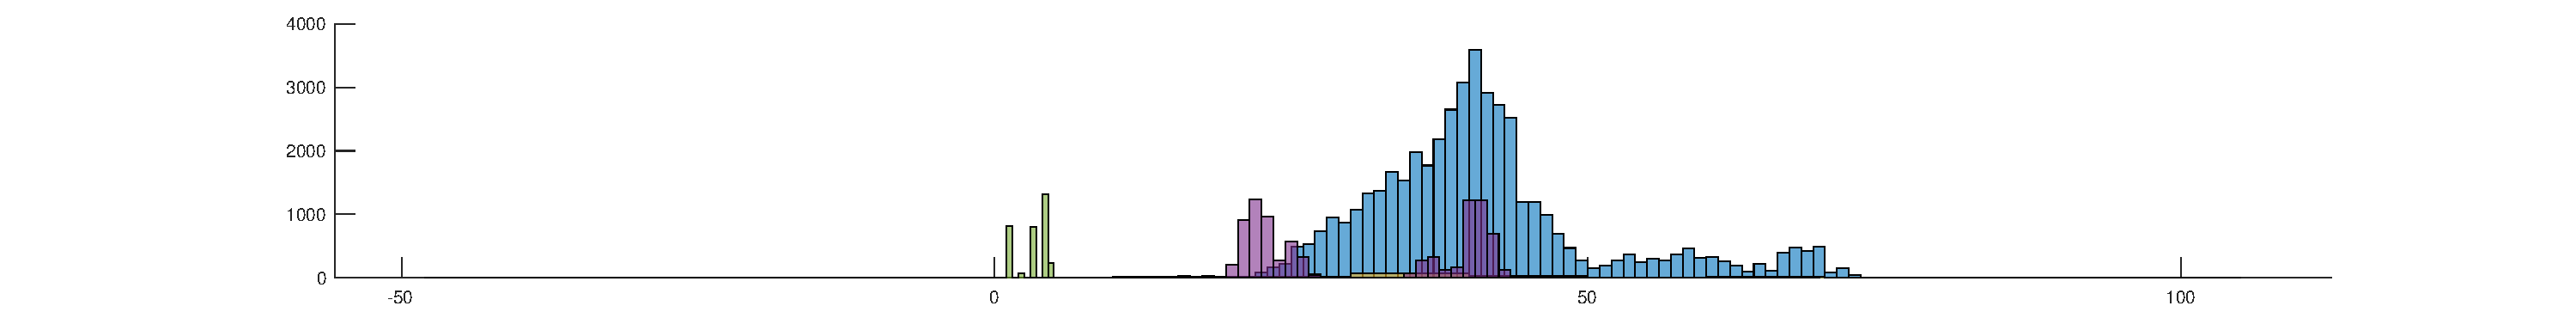
\includegraphics[width=\textwidth]{../src/figures/fssvm/shuttle_hist_7}}
\caption{3 out of 9 features of the Shuttle dataset. 48.586, 50, 171, 8903, 3267, 10 and 13 samples belong to class 1, 2, 3, 4, 5, 6 and 7 respectively. The class names are Rad Flow, Fpv Close, Fpv Open, High, Bypass, Bpv Close, Bpv Open.}
\label{shuttlehist}
\end{figure}

Rather than using the \texttt{sign} function a rounding was applied to obtain a class. This gave much better results, into the mid 90\% (estimates based on a train \& test split are shown in figure \ref{shuttleestimates}). One of the parameters that can be tuned is $k$. It specifies the number of prototype vectors indirectly ($M=k\cdot\sqrt{N}$). As it increases the time needed to generate the model does, too, and of course the number of support vectors decreases (certainly so for the classical FS-SVM models). Up until a certain point increasing $k$ also decreases the error rate. Yet another example of a bias-variance tradeoff relating to the complexity of the model. The required time for model generation doesn't differ much for the strategies with or without post-processing. This mirrors the result of the study introducing the latter (the same holds for the windowing discussed there, too).

\begin{figure}[!htb]
\centering
\begin{minipage}{\textwidth}
        \centering
        \subfloat[Error estimation.]{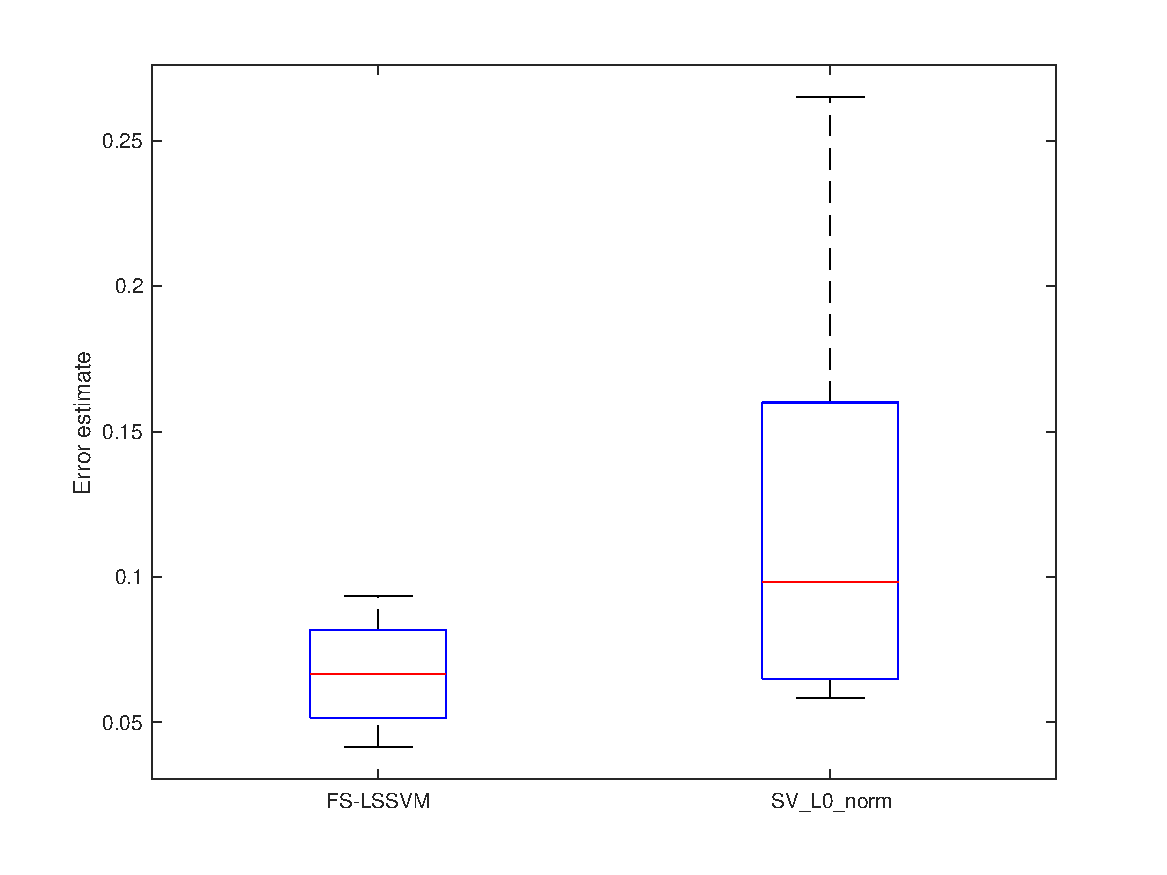
\includegraphics[width=0.32\textwidth]{../src/figures/fssvm/shuttle_comparison_error_2}}\hfil
	\subfloat[Estimation of the number of support vectors.]{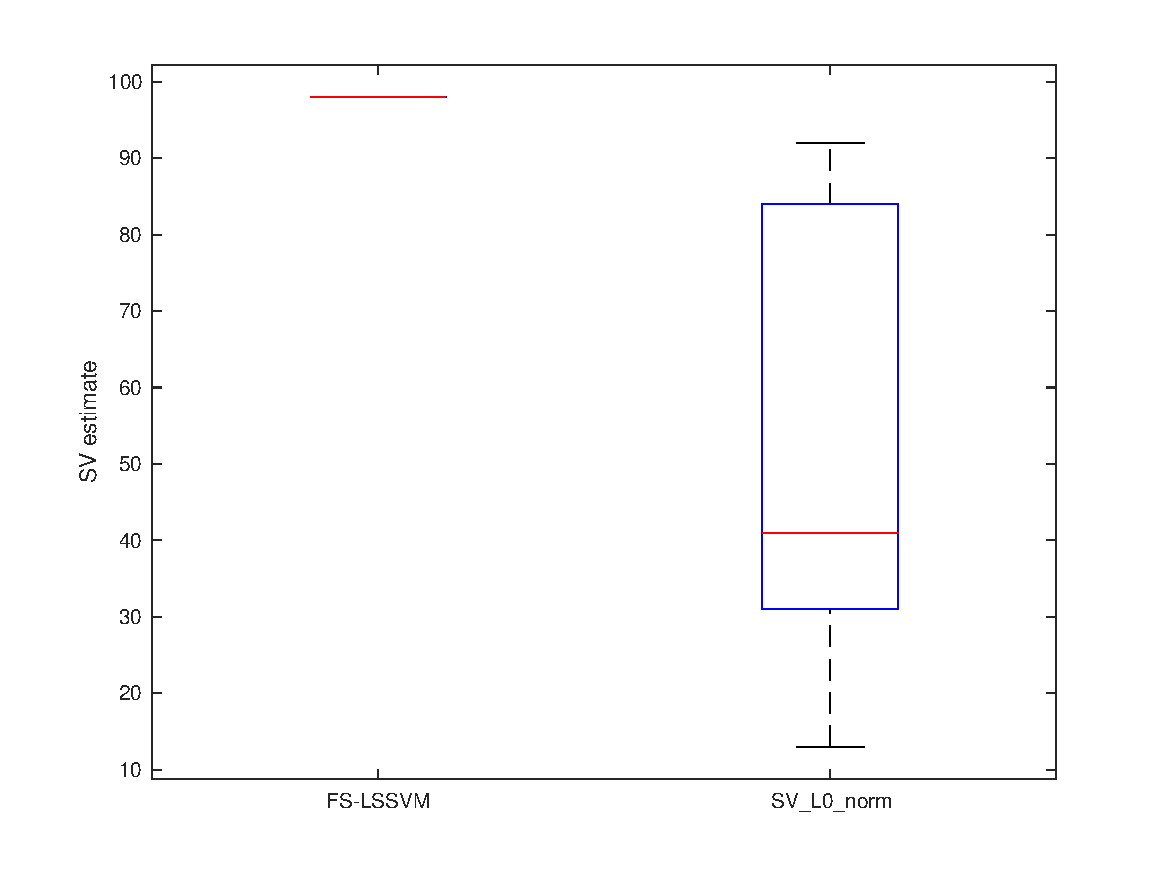
\includegraphics[width=0.32\textwidth]{../src/figures/fssvm/shuttle_comparison_sv_2}}\hfil
	\subfloat[Time estimation.]{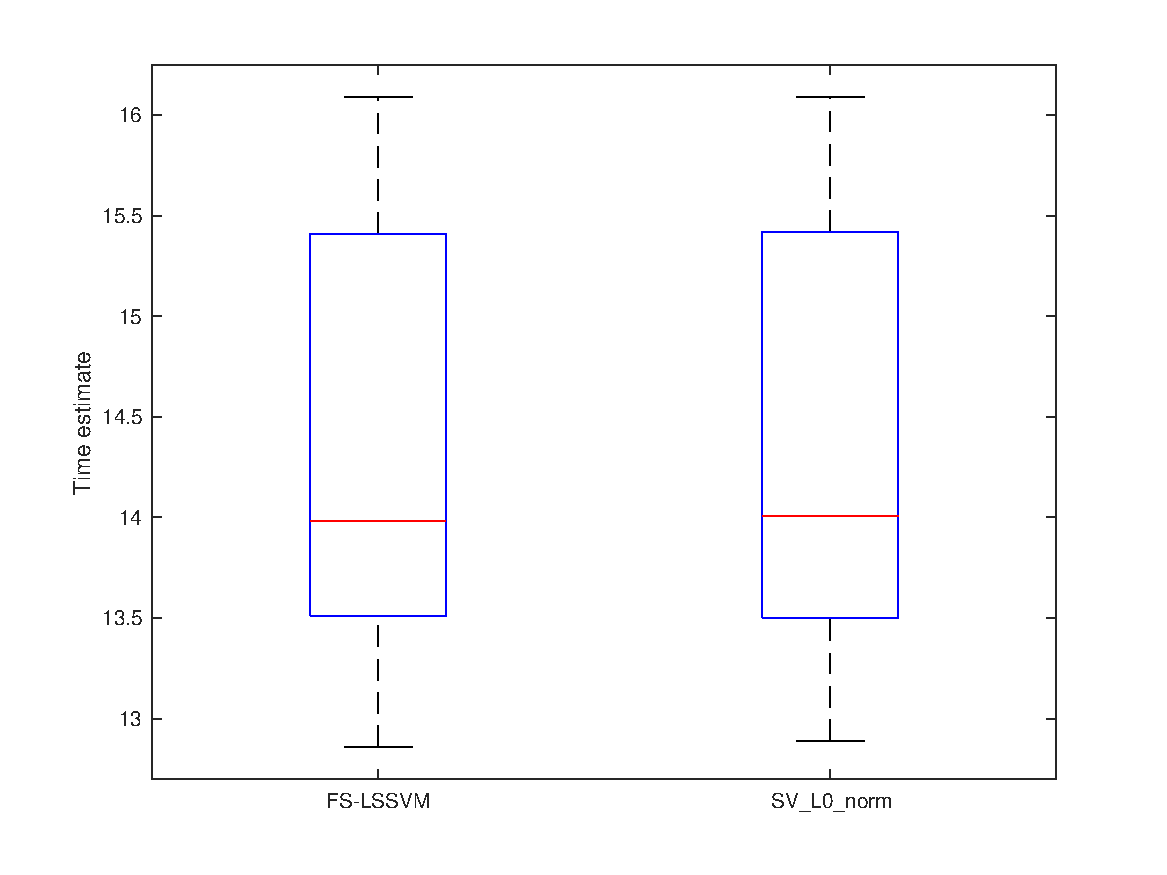
\includegraphics[width=0.32\textwidth]{../src/figures/fssvm/shuttle_comparison_time_2}}\hfil
	\caption*{$k=2$}
\end{minipage}
\begin{minipage}{\textwidth}
        \centering
        \subfloat[Error estimation.]{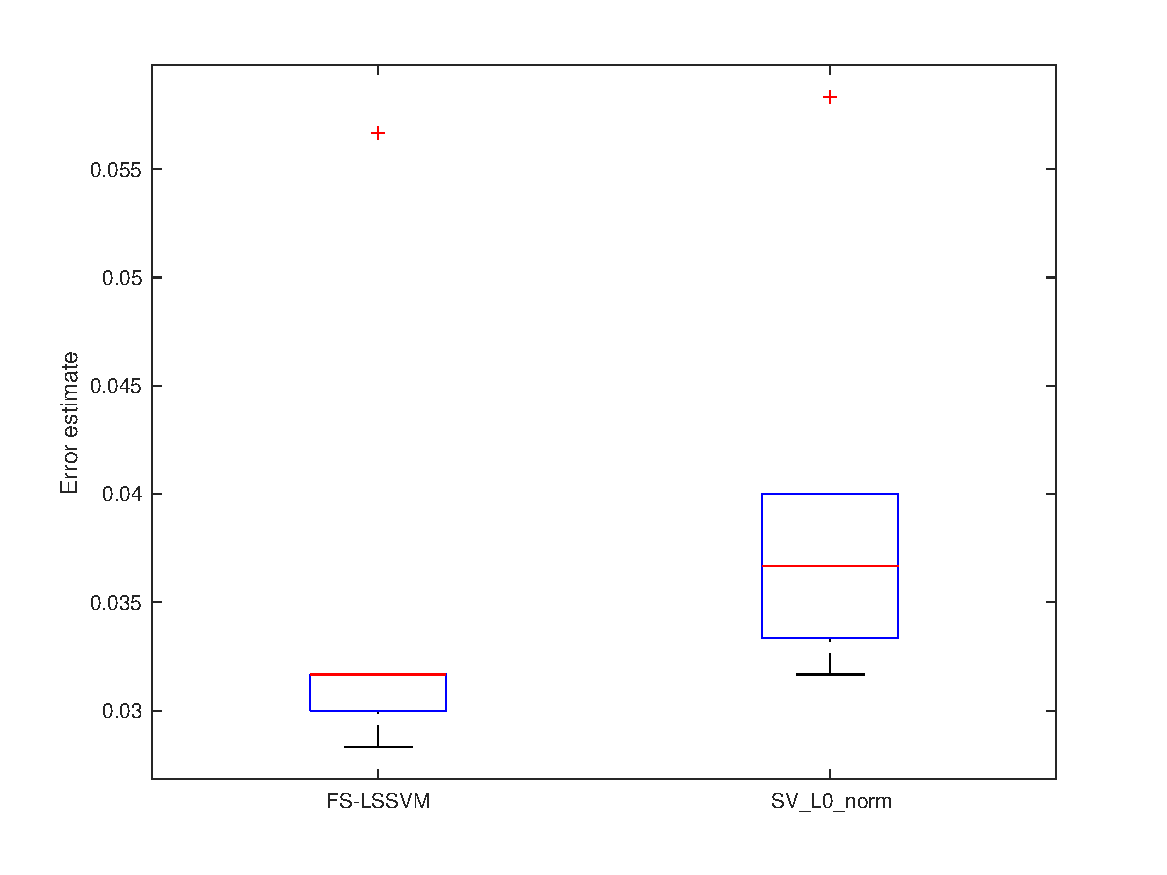
\includegraphics[width=0.32\textwidth]{../src/figures/fssvm/shuttle_comparison_error_4}}\hfil
	\subfloat[Estimation of the number of support vectors.]{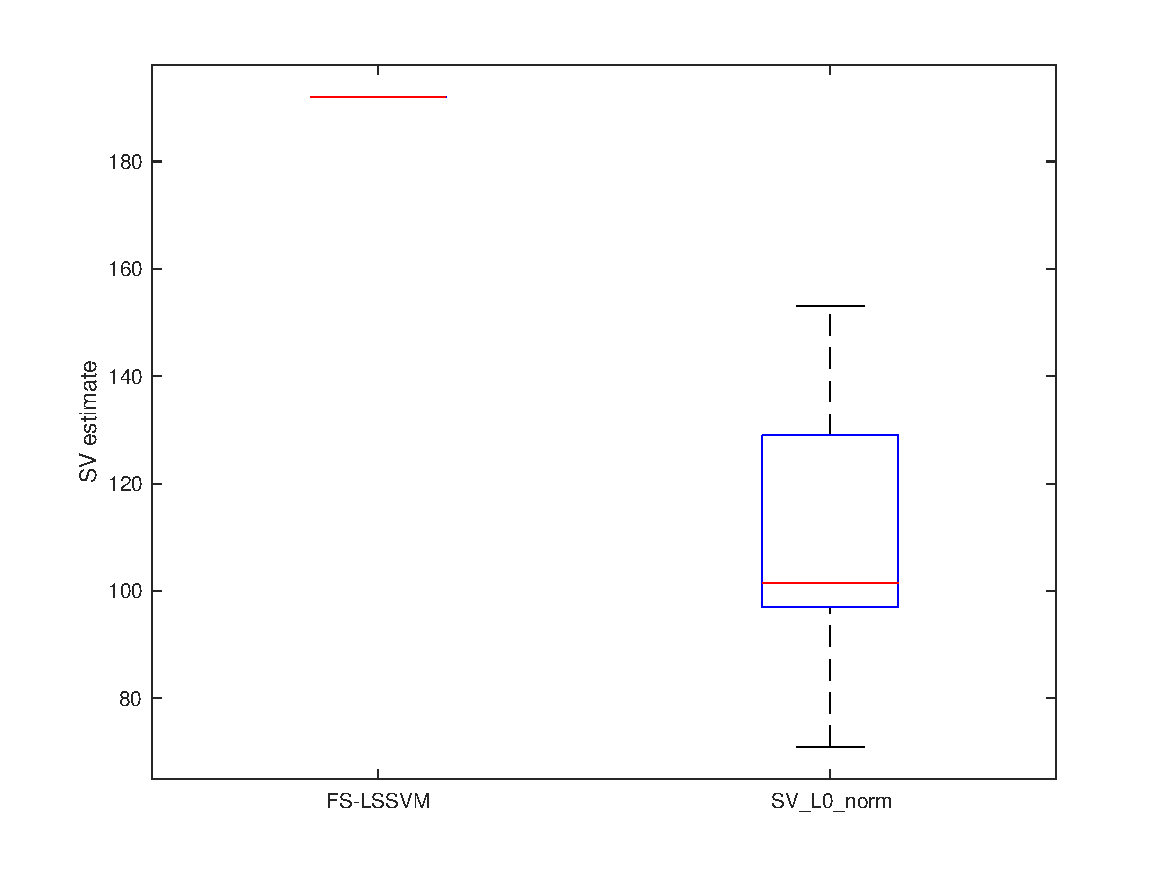
\includegraphics[width=0.32\textwidth]{../src/figures/fssvm/shuttle_comparison_sv_4}}\hfil
	\subfloat[Time estimation.]{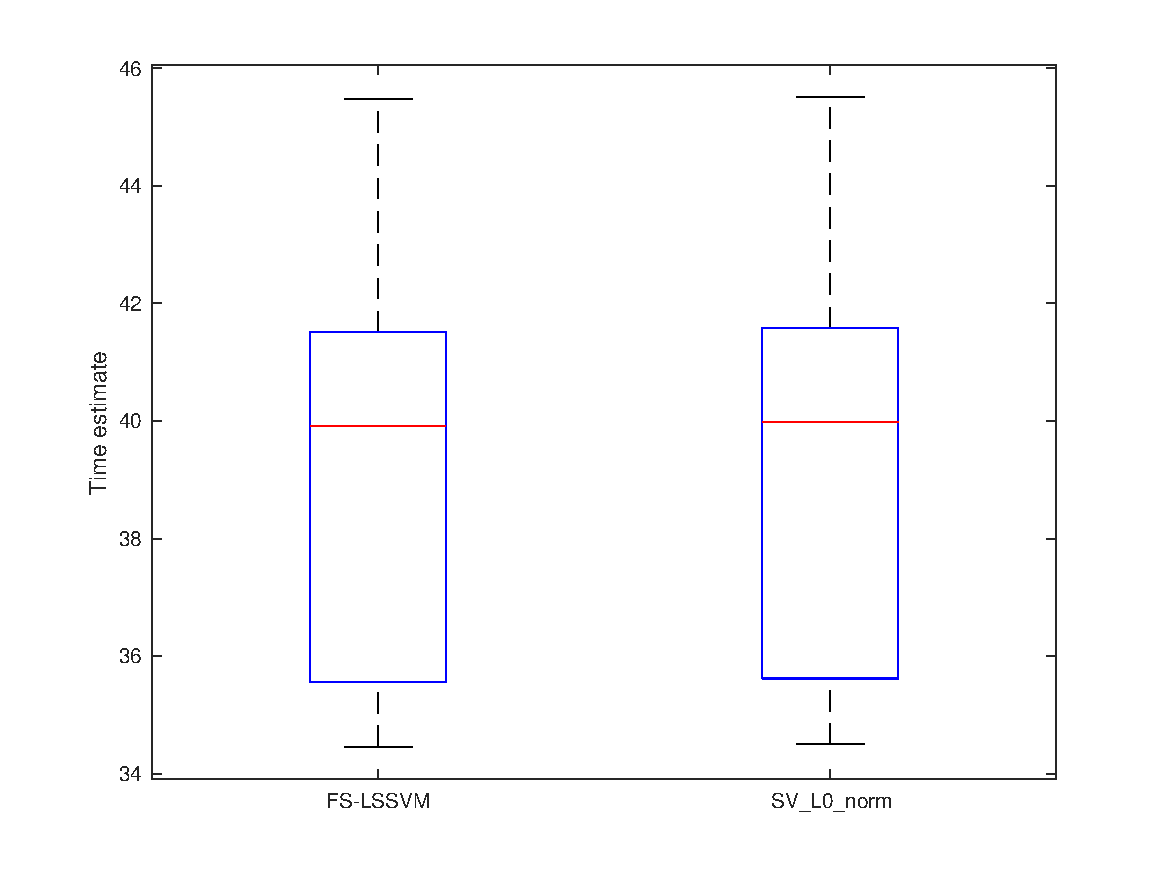
\includegraphics[width=0.32\textwidth]{../src/figures/fssvm/shuttle_comparison_time_4}}\hfil
	\caption*{$k=4$}
\end{minipage}
\begin{minipage}{\textwidth}
        \centering
        \subfloat[Error estimation.]{\includegraphics[width=0.32\textwidth]{../src/figures/fssvm/shuttle_comparison_error_6}}\hfil
	\subfloat[Estimation of the number of support vectors.]{\includegraphics[width=0.32\textwidth]{../src/figures/fssvm/shuttle_comparison_sv_6}}\hfil
	\subfloat[Time estimation.]{\includegraphics[width=0.32\textwidth]{../src/figures/fssvm/shuttle_comparison_time_6}}\hfil
	\caption*{$k=6$}
\end{minipage}
\begin{minipage}{\textwidth}
        \centering
        \subfloat[Error estimation.]{\includegraphics[width=0.32\textwidth]{../src/figures/fssvm/shuttle_comparison_error_8}}\hfil
	\subfloat[Estimation of the number of support vectors.]{\includegraphics[width=0.32\textwidth]{../src/figures/fssvm/shuttle_comparison_sv_8}}\hfil
	\subfloat[Time estimation.]{\includegraphics[width=0.32\textwidth]{../src/figures/fssvm/shuttle_comparison_time_8}}\hfil
	\caption*{$k=8$}
\end{minipage}
\caption{Boxplots for estimates of the error, number of support vectors and time needed to generate FS-SVMs with or without $\ell_0$ norm post-processing procedure. Estimates are based on results on a test set (20\% of 3000 samples). Estimates based on 10-fold cross-validation are about equivalent. The dataset is restricted to 3000 samples to avoid long runtimes. These belong to the first 5 classes. At all times an RBF kernel is used as a linear kernel isn't supported.}
\label{shuttleestimates}
\end{figure}

\fakesubsubsection{California housing dataset}{}

The California housing dataset contains information about block groups in California. Features include such things as median income, mean number of rooms in houses, ... and the dependent variable is the median house value. In other words, a 10-dimensional regression problem.
